\documentclass[11pt,a4paper]{article}
\usepackage[T1]{fontenc}
\usepackage[utf8]{inputenc}
\usepackage{lmodern,microtype}
\usepackage{geometry}
\geometry{top=24mm,bottom=25mm,left=23mm,right=23mm}
\usepackage{amsmath,amssymb,amsthm,mathtools,bm,mathrsfs}
\usepackage{booktabs,array,longtable,enumitem,multicol,graphicx,float}
\usepackage[most]{tcolorbox}
\usepackage{fancyhdr,lastpage,xcolor,hyperref,cleveref,titlesec,needspace}
\usepackage{pgfplots}
\pgfplotsset{compat=1.18}
\definecolor{navy}{HTML}{172B4D}
\definecolor{teal}{HTML}{087E83}
\definecolor{ink}{HTML}{263849}
\definecolor{pale}{HTML}{F0F6F8}
\definecolor{line}{HTML}{C9D9E0}
\hypersetup{colorlinks=true,linkcolor=navy,citecolor=teal,urlcolor=teal,
 pdftitle={Quantum Mechanics I Assignment IV: Complete Problems and Worked Solutions},
 pdfauthor={Mathematical Physics Study Manuscript},
 pdfsubject={Spherical symmetry, hydrogen atom, spherical wells, angular momentum algebra and conservation}}
\setlength{\parindent}{0pt}\setlength{\parskip}{4.5pt}\emergencystretch=3em
\setlength{\headheight}{16pt}
\pagestyle{fancy}\fancyhf{}
\fancyhead[L]{\small\sffamily QUANTUM MECHANICS I \textbar{} ASSIGNMENT IV}
\fancyhead[R]{\small\sffamily M.Sc. MATHEMATICAL PHYSICS}
\fancyfoot[L]{\footnotesize\sffamily Pedagogical preprint \textbullet{} worked solutions}
\fancyfoot[R]{\small\thepage\ / \pageref{LastPage}}
\renewcommand{\headrulewidth}{0.35pt}
\titleformat{\section}{\Large\bfseries\color{navy}}{\thesection.}{0.7em}{}
\titleformat{\subsection}{\large\bfseries\color{navy}}{\thesubsection}{0.7em}{}
\titleformat{\subsubsection}{\normalsize\bfseries\color{teal}}{}{0pt}{}
\titlespacing*{\section}{0pt}{18pt}{9pt}
\titlespacing*{\subsection}{0pt}{14pt}{6pt}
\tcbset{colback=pale,colframe=line,arc=1mm,boxrule=0.55pt,left=8pt,right=8pt,top=7pt,bottom=7pt}
\newtcolorbox{questionbox}{breakable,colback=white,colframe=teal,boxrule=.7pt,title={\footnotesize\sffamily ASSIGNMENT PROBLEM},fonttitle=\bfseries,coltitle=teal,boxed title style={colback=white,colframe=white},attach boxed title to top left={yshift=-2mm,xshift=5mm}}
\newtcolorbox{resultbox}{breakable,colback=pale,colframe=teal,boxrule=.7pt}
\newcommand{\key}[1]{\begin{resultbox}\centering\(\displaystyle #1\)\end{resultbox}}
\newcommand{\dd}{\mathrm{d}}
\newcommand{\iu}{\mathrm{i}}
\newcommand{\ee}{\mathrm{e}}
\newcommand{\avg}[1]{\left\langle #1\right\rangle}
\newcommand{\ket}[1]{\left|#1\right\rangle}
\newcommand{\bra}[1]{\left\langle #1\right|}
\newcommand{\braket}[2]{\left\langle #1\middle|#2\right\rangle}
\newcommand{\norm}[1]{\left\lVert #1\right\rVert}
\newcommand{\p}{\partial}
\newcommand{\R}{\mathbb R}
\newcommand{\Hh}{\mathcal H}
\newcommand{\aH}{a_{\mathrm H}}
\newcommand{\mH}{\mu_{\mathrm H}}
\newcommand{\eps}{\varepsilon_0}
\newcommand{\lap}{\nabla^2}
\newcommand{\Lop}{\hat{\mathbf L}}
\newcommand{\op}[1]{\hat{#1}}
\allowdisplaybreaks[2]
\begin{document}
\begin{titlepage}
\thispagestyle{empty}
\vspace*{14mm}
{\color{teal}\rule{\textwidth}{1.5pt}}\\[11mm]
{\sffamily\fontsize{29}{34}\selectfont\bfseries Quantum Mechanics--I:\\[2mm] Assignment IV}\par
\vspace{7mm}
{\sffamily\Large Complete Problems and Step-by-Step Mathematical Solutions}\par
\vspace{10mm}
{\large\bfseries 23 problems: Part A (10) and Part B (13)}\par
\vspace{8mm}
\begin{tcolorbox}[colback=pale,colframe=teal]
\textbf{Source:} Department of Physics \& Nanotechnology, SRM Institute of Science and Technology (SRMIST), Kattankulathur. M.Sc. Physics / M.Sc. Applied Physics, Semester I. Quantum Mechanics--I (PPY25103J) / Quantum Mechanics (PAP25103J), Assignment--IV.\\[4pt]
\textbf{Topics:} Coulomb symmetry, single-valued wavefunctions, normalized spherical harmonics, hydrogen spectra, angular momentum operator identities, separation of variables, infinite spherical well, hydrogen radial equation, exact expectation values, ladder algebra, and Noether/Heisenberg conservation laws.
\end{tcolorbox}
\vspace{10mm}
{\Large\bfseries\color{navy} Mathematical Physics Study Manuscript}\par
\vspace{4mm}
{\normalsize Problem statement \(\longrightarrow\) full derivation \(\longrightarrow\) verification \(\longrightarrow\) exam-ready conclusion}\par
\vfill
{\large November 2026}\par\vspace{4mm}
{\small arXiv-inspired \LaTeX{} layout; educational compilation, not a submitted or peer-reviewed research article.}\par
\vspace{9mm}{\color{teal}\rule{\textwidth}{1.5pt}}
\end{titlepage}
\begin{abstract}
This complete mathematical-physics study manuscript presents all ten Part A problems and all thirteen Part B problems in SRMIST Quantum Mechanics--I Assignment IV. The questions are typeset from the provided course sheet and remain in their original order. The solutions follow the detailed first-principles derivations developed in the study discussion, with self-contained calculations, correct boundary conditions, Hilbert-space qualifications, explicit radial integrations, algebraic angular momentum calculations, and concise exam-ready conclusions. An analytic vector plot of the hydrogen radial probability density is included. The text is an edited LaTeX re-typesetting and synthesis, not a claim that every word of earlier chat answers has been reproduced verbatim. Where the printed sheet adopts a convention-dependent identity for spherical harmonics, the convention and standard alternative are both explained. This document is a pedagogical manuscript rather than an original research submission.
\end{abstract}
{\small\setlength{\parskip}{0pt}\tableofcontents}
\clearpage
\section{Source, conventions, and scope}
\textbf{Assignment source.} The two-page \emph{Assignment IV} section of \texttt{QM-AS-1-5.pdf} gives Part A, Problems 1--10, and Part B, Problems 1--13. The question boxes below preserve the problem order and mathematical content, with normalized LaTeX typography. All solutions are elaborated at M.Sc. level; additional checks and comments are clearly within the solutions rather than changes to the assigned questions.

\textbf{Notation.} We use \(\hbar=h/(2\pi)\), \(\mathbf p=-\iu\hbar\nabla\), \([x_i,p_j]=\iu\hbar\delta_{ij}\), \(L_i=\varepsilon_{ijk}x_jp_k\), and \(L_\pm=L_x\pm\iu L_y\). The electron--proton reduced mass is \(\mH=m_em_p/(m_e+m_p)\), and \(\aH=4\pi\eps\hbar^2/(\mH e^2)\) is the reduced-mass Bohr-radius scale. For one-electron ions with nuclear charge \(Z\), use \(\mu_Z\) and \(a_Z=4\pi\eps\hbar^2/(\mu_ZZe^2)\). Standard spherical harmonics are given in the Condon--Shortley convention unless a question explicitly asks for a different rephasing.

\textbf{Rigor.} Differential-operator commutators are established on suitable smooth common invariant cores and interpreted on physical self-adjoint domains. Probability moments are assumed finite. For central potentials, rotational invariance includes the relevant boundary conditions and Hamiltonian domain. The angular quantum number for ordinary scalar orbital wavefunctions is an integer, while the abstract angular momentum algebra admits half-integer representations.

\section{Part A: short-answer problems (1--10)}
\subsection{A1. Spherical symmetry of the Coulomb interaction}
\begin{questionbox}What is meant by spherical symmetry of the Coulombic interaction?\end{questionbox}
For point charges \(q_1,q_2\), the interaction depends only on their separation:
\begin{equation}V(\mathbf r)=\frac{q_1q_2}{4\pi\eps|\mathbf r|}=:V(r).\end{equation}
For electron--proton attraction, \(q_1q_2=-e^2\), hence \(V(r)=-e^2/(4\pi\eps r)\). A three-dimensional rotation \(\mathcal R\in SO(3)\) preserves Euclidean length: \(|\mathcal R\mathbf r|=|\mathbf r|\). Consequently
\begin{equation}V(\mathcal R\mathbf r)=V(\mathbf r),\qquad \nabla V(r)=\frac{\dd V}{\dd r}\,\hat{\mathbf r}.\end{equation}
The force \(\mathbf F=-\nabla V\) is central (radial), with no preferred direction. Quantum mechanically the scalar Hamiltonian \(H=p^2/(2\mu)+V(r)\) is rotation-invariant and therefore \([H,L_i]=0\), a fact proved in detail in B13.
\key{\boxed{V(\mathcal R\mathbf r)=V(\mathbf r)\quad\forall\mathcal R\in SO(3).}}
\textbf{Exam-ready conclusion.} Coulombic interaction is spherically symmetric because the potential depends only on the relative distance \(r\), not on the angular orientation of \(\mathbf r\).

\subsection{A2. Integer-valued azimuthal quantum number}
\begin{questionbox}Given that the azimuthal part of the hydrogen atom wave function is \(\Phi(\phi)=e^{\iu m\phi}\), show that \(m\) can only take integer values.\end{questionbox}
Angles \(\phi\) and \(\phi+2\pi\) represent the same spatial point. An ordinary scalar orbital wavefunction must therefore satisfy \(\Phi(\phi+2\pi)=\Phi(\phi)\). Insert \(\Phi(\phi)=e^{\iu m\phi}\):
\begin{align}
e^{\iu m(\phi+2\pi)}&=e^{\iu m\phi},\\
e^{2\pi\iu m}&=1,\\
\cos(2\pi m)+\iu\sin(2\pi m)&=1.
\end{align}
The condition means \(2\pi m=2\pi k\) for some integer \(k\). Hence
\key{\boxed{m\in\mathbb Z=\{0,\pm1,\pm2,\ldots\}.}}
Normalized azimuthal functions are \(\Phi_m=(2\pi)^{-1/2}e^{\iu m\phi}\); \(\int_0^{2\pi}\Phi_m^*\Phi_{m'}\dd\phi=\delta_{mm'}\). For a fixed orbital \(l\), regularity of the polar solution additionally imposes \(-l\le m\le l\).

\subsection{A3. Orthonormality of spherical harmonics and hydrogen eigenstates}
\begin{questionbox}Write the orthonormality condition for (i) spherical harmonic functions and (ii) hydrogen atom wave functions.\end{questionbox}
\textbf{(i) Angular functions.} The unit-sphere measure is \(\dd\Omega=\sin\theta\,\dd\theta\,\dd\phi\). Thus
\begin{equation}\boxed{\int_0^{2\pi}\!\int_0^\pi Y_l^{m*}(\theta,\phi)Y_{l'}^{m'}(\theta,\phi)\sin\theta\,\dd\theta\,\dd\phi=\delta_{ll'}\delta_{mm'}.}\end{equation}
\textbf{(ii) Hydrogen eigenfunctions.} With \(\psi_{nlm}=R_{nl}(r)Y_l^m(\theta,\phi)\) and \(\dd^3r=r^2\dd r\,\dd\Omega\), orthonormality of bound states is
\begin{equation}\boxed{\int_{\mathbb R^3}\psi_{nlm}^*(\mathbf r)\psi_{n'l'm'}(\mathbf r)\,\dd^3r=\delta_{nn'}\delta_{ll'}\delta_{mm'}.}\end{equation}
The radial normalization is \(\int_0^\infty|R_{nl}(r)|^2r^2\dd r=1\); for the same \(l\), orthogonality of distinct radial bound states gives \(\int_0^\infty R_{nl}^*R_{n'l}\,r^2\dd r=\delta_{nn'}\). Continuum Coulomb states instead require delta-normalization and are not covered by the discrete Kronecker-delta statement.

\subsection{A4. Complex conjugation and spherical harmonic phase conventions}
\begin{questionbox}Show that \(Y_l^{-m}=(Y_l^m)^*\). \emph{This is the identity printed on the assignment sheet.}\end{questionbox}
This relation depends on the relative phase chosen for the negative-\(m\) basis functions. For any normalized complex harmonic, the complex conjugate transforms under \(L_z=-\iu\hbar\partial_\phi\) with magnetic quantum number \(-m\), and under \(L^2\) with the same \(l(l+1)\). For fixed \((l,-m)\), that eigenspace is one-dimensional, so conjugation is proportional to \(Y_l^{-m}\), with a phase of modulus one. One may \emph{define} the phases of the negative-\(m\) harmonics so that
\begin{equation}\boxed{Y_l^{-m}=(Y_l^m)^*.}\end{equation}
\textbf{Important convention clarification.} In the more common Condon--Shortley convention used for the explicitly normalized harmonics and standard positive ladder coefficients in this manuscript,
\begin{equation}\boxed{Y_l^{-m}=(-1)^m(Y_l^m)^*.}\end{equation}
For example \(Y_1^1=-\sqrt{3/(8\pi)}\sin\theta e^{\iu\phi}\), while \(Y_1^{-1}=+\sqrt{3/(8\pi)}\sin\theta e^{-\iu\phi}\): the minus sign matters. The assignment's printed formula is recovered by rephasing the negative-\(m\) states: \(\widetilde Y_l^{-m}=(-1)^mY_l^{-m}\) (for \(m>0\)); then \(\widetilde Y_l^{-m}=(Y_l^m)^*\). The rephasing does not change eigenvalues or probabilities but changes some ladder coefficients' signs. These conventions must not be silently mixed.

\subsection{A5. Quantized energies of hydrogen and hydrogenic ions}
\begin{questionbox}Write the energy quantization formula for (i) hydrogen atom and (ii) a hydrogenic atom.\end{questionbox}
\textbf{Hydrogen (\(Z=1\)).} Define \(g=e^2/(4\pi\eps)\), \(\mH=m_em_p/(m_e+m_p)\). Separation of the Coulomb radial equation and polynomial termination yield
\begin{equation}\boxed{E_n^{\rm H}=-\frac{\mH e^4}{2(4\pi\eps)^2\hbar^2n^2},\qquad n=1,2,3,\ldots}\end{equation}
In the fixed-proton approximation this is \(E_n\simeq-13.6057\,\mathrm{eV}/n^2\), usually rounded to \(-13.6\,\mathrm{eV}/n^2\); with proton reduced mass the scale is about \(13.5983\,\mathrm{eV}\).

\textbf{Hydrogenic (one-electron) ion of nuclear charge \(+Ze\).} Its potential is \(V_Z(r)=-Ze^2/(4\pi\eps r)\). Let \(\mu_Z\) be its electron--nucleus reduced mass. Then
\begin{equation}\boxed{E_n^{(Z)}=-\frac{\mu_Z Z^2e^4}{2(4\pi\eps)^2\hbar^2n^2}.}\end{equation}
For a heavy nucleus, \(\mu_Z\simeq m_e\), yielding \(E_n^{(Z)}\simeq-13.6Z^2/n^2\,\mathrm{eV}\). Nuclear size, relativity, radiative effects and electronic correlations are outside the ideal Coulomb model. Full derivation: B5.

\subsection{A6. Ground-state wavefunctions of hydrogen and hydrogenic ions}
\begin{questionbox}Write the ground-state wave function for (i) hydrogen atom and (ii) a hydrogenic atom.\end{questionbox}
For an attractive Coulomb potential \(-g/r\), the bound \(1s\) solution (\(n=1,l=m=0\)) has radial dependence \(e^{-r/a}\), where \(a=\hbar^2/(\mu g)\). Spherical normalization gives
\begin{align}
1&=|C|^2\int_{\R^3}\ee^{-2r/a}\dd^3r=4\pi|C|^2\int_0^\infty r^2\ee^{-2r/a}\dd r\\
&=4\pi|C|^2\frac{2!}{(2/a)^3}=\pi a^3|C|^2.
\end{align}
Choosing \(C>0\), \(C=(\pi a^3)^{-1/2}\). For hydrogen \(a=\aH=4\pi\eps\hbar^2/(\mH e^2)\), so
\begin{equation}\boxed{\psi_{100}^{\rm H}(r)=\frac1{\sqrt{\pi\aH^3}}\ee^{-r/\aH}.}\end{equation}
For nuclear charge \(Z\) and nuclear mass \(M_Z\), \(\mu_Z=m_eM_Z/(m_e+M_Z)\) and \(a_Z=4\pi\eps\hbar^2/(\mu_ZZe^2)\). Hence
\begin{equation}\boxed{\psi_{100}^{(Z)}(r)=\frac1{\sqrt{\pi a_Z^3}}\ee^{-r/a_Z}.}\end{equation}
Alternatively, setting \(a_{\mu,Z}=4\pi\eps\hbar^2/(\mu_Z e^2)\), this is \(\psi_{100}^{(Z)}=(Z^3/(\pi a_{\mu,Z}^3))^{1/2}\ee^{-Zr/a_{\mu,Z}}\). The wavefunctions are full three-dimensional spatial states and include \(Y_0^0=1/\sqrt{4\pi}\). Their radial parts are \(R_{10}=2a^{-3/2}\ee^{-r/a}\).

\subsection{A7. Short note on the hydrogen spectrum}
\begin{questionbox}Write a short note on hydrogen spectrum.\end{questionbox}
The discrete bound-state energies in the nonrelativistic Coulomb model are
\begin{equation}E_n=-\frac{\mH e^4}{2(4\pi\eps)^2\hbar^2n^2}=-\frac{E_{\rm Ry,H}}{n^2},\qquad n\ge1.\end{equation}
An emitted photon from a transition \(n_i>n_f\) has energy \(h\nu=E_{n_i}-E_{n_f}\). Thus
\begin{equation}\boxed{\frac1\lambda=R_{\rm H}\left(\frac1{n_f^2}-\frac1{n_i^2}\right),\quad n_i>n_f,}\end{equation}
where \(R_{\rm H}=\mu_{\rm H}e^4/[8\eps^2h^3c]\) is the reduced-mass-corrected Rydberg constant. The Lyman series ends on \(n_f=1\) (ultraviolet), Balmer on \(n_f=2\) (some visible lines), Paschen on \(n_f=3\) (infrared), and Brackett/Pfund on \(n_f=4,5\) (infrared). The levels approach the ionization threshold \(E=0\) as \(n\to\infty\), and line spacings narrow near series limits. For electric-dipole transitions the orbital selection rules are \(\Delta l=\pm1\) and \(\Delta m=0,\pm1\). These spectra are further modified in real hydrogen by fine structure, hyperfine structure, Lamb shifts and finite proton mass.

\subsection{A8. Seven orbital-angular-momentum commutators}
\begin{questionbox}
Prove the following commutators:
\begin{align*}
[\hat L_x,\hat L_y]&=\iu\hbar\hat L_z,\\
[\hat L^2,\hat L_x]&=[\hat L^2,\hat L_y]=[\hat L^2,\hat L_z]=0,\\
[\hat L_z,\hat z]&=0,\quad [\hat L_z,\hat p_z]=0,\\
[\hat L^2,\hat L_\pm]&=0,\quad [\hat L_z,\hat L_\pm]=\pm\hbar\hat L_\pm,\\
[\hat L_+,\hat L_-]&=2\hbar\hat L_z.
\end{align*}
\end{questionbox}
Use the canonical relations \([x_i,p_j]=\iu\hbar\delta_{ij}\), \([x_i,x_j]=[p_i,p_j]=0\), and \([A,BC]=[A,B]C+B[A,C]\).

\textbf{(1) Cartesian angular commutator.} The components are \(L_x=yp_z-zp_y\), \(L_y=zp_x-xp_z\), \(L_z=xp_y-yp_x\). Expand:
\begin{align}
[L_x,L_y]&=[yp_z,zp_x]-[yp_z,xp_z]-[zp_y,zp_x]+[zp_y,xp_z]\\
&=(-\iu\hbar yp_x)+0+0+(\iu\hbar xp_y)\\
&=\iu\hbar(xp_y-yp_x)=\boxed{\iu\hbar L_z}.
\end{align}
In the first term, \([yp_z,zp_x]=y[p_z,z]p_x=-\iu\hbar yp_x\); in the last term \([zp_y,xp_z]=[z,p_z]xp_y=\iu\hbar xp_y\). Cyclic permutations give \([L_y,L_z]=\iu\hbar L_x\) and \([L_z,L_x]=\iu\hbar L_y\).

\textbf{(2) Casimir commutators.} For instance,
\begin{align}
[L^2,L_z]&=[L_x^2,L_z]+[L_y^2,L_z]\\
&=-\iu\hbar(L_xL_y+L_yL_x)+\iu\hbar(L_yL_x+L_xL_y)=0.
\end{align}
Cycling the indices proves \(\boxed{[L^2,L_x]=[L^2,L_y]=[L^2,L_z]=0}\).

\textbf{(3) Longitudinal position.} Since \(L_z=xp_y-yp_x\),
\begin{equation}[L_z,z]=x[p_y,z]-y[p_x,z]+[x,z]p_y-[y,z]p_x=\boxed0.\end{equation}

\textbf{(4) Longitudinal momentum.} Similarly,
\begin{equation}[L_z,p_z]=x[p_y,p_z]-y[p_x,p_z]+[x,p_z]p_y-[y,p_z]p_x=\boxed0.\end{equation}

\textbf{(5) Casimir and ladders.} From \(L_\pm=L_x\pm\iu L_y\),
\begin{equation}[L^2,L_\pm]=[L^2,L_x]\pm\iu[L^2,L_y]=\boxed0.\end{equation}

\textbf{(6) \(z\)-component and ladders.} Using \([L_z,L_x]=\iu\hbar L_y\), \([L_z,L_y]=-\iu\hbar L_x\),
\begin{align}
[L_z,L_+]&=\iu\hbar L_y+\iu(-\iu\hbar L_x)=\hbar L_+,\\
[L_z,L_-]&=\iu\hbar L_y-\iu(-\iu\hbar L_x)=-\hbar L_-.
\end{align}
Hence \(\boxed{[L_z,L_\pm]=\pm\hbar L_\pm}\).

\textbf{(7) Ladder commutator.}
\begin{align}
[L_+,L_-]&=[L_x+\iu L_y,L_x-\iu L_y]\\
&=-\iu[L_x,L_y]+\iu[L_y,L_x]\\
&=-2\iu(\iu\hbar L_z)=\boxed{2\hbar L_z}.
\end{align}
These identities are operator equalities on an appropriate common invariant dense domain; they do not require a particular state.

\subsection{A9. Factorization of \texorpdfstring{$L^2$}{L2} with raising/lowering operators}
\begin{questionbox}Show that \(\hat L^2=\hat L_\pm\hat L_\mp+\hat L_z^2\mp\hbar\hat L_z\).\end{questionbox}
Compute the ordered products, taking care that \(L_x\) and \(L_y\) do not commute:
\begin{align}
L_+L_-&=(L_x+\iu L_y)(L_x-\iu L_y)\\
&=L_x^2+L_y^2-\iu[L_x,L_y]\\
&=L^2-L_z^2+\hbar L_z.
\end{align}
Therefore \(\boxed{L^2=L_+L_-+L_z^2-\hbar L_z}\). Likewise,
\begin{align}
L_-L_+&=(L_x-\iu L_y)(L_x+\iu L_y)\\
&=L_x^2+L_y^2+\iu[L_x,L_y]\\
&=L^2-L_z^2-\hbar L_z,
\end{align}
so \(\boxed{L^2=L_-L_++L_z^2+\hbar L_z}\). Combined:
\key{\boxed{L^2=L_\pm L_\mp+L_z^2\mp\hbar L_z.}}
As a check, subtract the product formulas to recover \([L_+,L_-]=2\hbar L_z\). See B11 for the role of these identities in proving spectral quantization.

\subsection{A10. Normalized angular-momentum ladder coefficients}
\begin{questionbox}The raising and lowering operators change the value of \(m\) by one unit: \(\hat L_\pm f_l^m=A_l^m f_l^{m\pm1}\). Using the equation in Q9, prove that the appropriate coefficient is \(A_l^m=\hbar\sqrt{l(l+1)-m(m\pm1)}\).\end{questionbox}
Use normalized angular eigenstates \(f_l^m=\ket{l,m}\) with
\begin{equation}L^2\ket{l,m}=\hbar^2l(l+1)\ket{l,m},\qquad L_z\ket{l,m}=\hbar m\ket{l,m}.\end{equation}
Suppose \(L_+\ket{l,m}=A_{lm}^{(+)}\ket{l,m+1}\). Because \(L_+^\dagger=L_-\), the squared norm is
\begin{align}
|A_{lm}^{(+)}|^2&=\norm{L_+\ket{l,m}}^2=\bra{l,m}L_-L_+\ket{l,m}\\
&=\bra{l,m}(L^2-L_z^2-\hbar L_z)\ket{l,m}\\
&=\hbar^2[l(l+1)-m(m+1)].
\end{align}
Similarly,
\begin{align}
|A_{lm}^{(-)}|^2&=\norm{L_-\ket{l,m}}^2=\bra{l,m}L_+L_-\ket{l,m}\\
&=\hbar^2[l(l+1)-m(m-1)].
\end{align}
Choose the usual relative phases (Condon--Shortley) so that coefficients are real and nonnegative:
\key{\boxed{L_\pm\ket{l,m}=\hbar\sqrt{l(l+1)-m(m\pm1)}\ket{l,m\pm1}.}}
Equivalent factorizations are \(\hbar\sqrt{(l-m)(l+m+1)}\) for raising and \(\hbar\sqrt{(l+m)(l-m+1)}\) for lowering. The coefficients vanish at \(m=l\) and \(m=-l\), respectively. The norms fix magnitudes, while the phase convention fixes signs. This completes Part A.

\clearpage
\section{Part B: long-answer problems (1--13)}
\subsection{B1. Separation of the 3D Schr\"odinger equation for a central potential}
\begin{questionbox}Apply the variable separation method to Schr\"odinger's equation in 3D and derive the radial and the angular equations (\(\theta\) and \(\phi\)) for a spherically symmetric potential \(V(r)\).\end{questionbox}
\subsubsection*{Step 1: Three-dimensional stationary Schr\"odinger equation}
For a spinless particle of mass \(\mu\) in a radial potential \(V(r)\),
\begin{equation}-\frac{\hbar^2}{2\mu}\nabla^2\psi+V(r)\psi=E\psi,\qquad \psi\in L^2(\R^3).\end{equation}
The Laplacian in spherical coordinates follows from the Euclidean metric \(\dd s^2=\dd r^2+r^2\dd\theta^2+r^2\sin^2\theta\dd\phi^2\):
\begin{equation}\boxed{\nabla^2=\frac1{r^2}\p_r(r^2\p_r)+\frac1{r^2\sin\theta}\p_\theta(\sin\theta\p_\theta)+\frac1{r^2\sin^2\theta}\p_\phi^2.}\end{equation}
Its Jacobian is \(\dd^3r=r^2\sin\theta\dd r\dd\theta\dd\phi\). Multiplying the Schr\"odinger equation by \(-2\mu/\hbar^2\) gives
\begin{equation}\nabla^2\psi+\frac{2\mu}{\hbar^2}[E-V(r)]\psi=0.\end{equation}

\subsubsection*{Step 2: Product separation}
Choose
\begin{equation}\boxed{\psi(r,\theta,\phi)=R(r)\Theta(\theta)\Phi(\phi).}\end{equation}
Then
\begin{align}
&\frac{\Theta\Phi}{r^2}\frac{\dd}{\dd r}\left(r^2\frac{\dd R}{\dd r}\right)+\frac{R\Phi}{r^2\sin\theta}\frac{\dd}{\dd\theta}\left(\sin\theta\frac{\dd\Theta}{\dd\theta}\right)\\
&\qquad+\frac{R\Theta}{r^2\sin^2\theta}\frac{\dd^2\Phi}{\dd\phi^2}+\frac{2\mu}{\hbar^2}[E-V]R\Theta\Phi=0.
\end{align}
Divide by \(R\Theta\Phi\) and multiply by \(r^2\):
\begin{equation}\underbrace{\frac1R\frac{\dd}{\dd r}(r^2R')+\frac{2\mu r^2}{\hbar^2}(E-V)}_{\text{radial only}}+\underbrace{\frac1{\Theta\sin\theta}\frac{\dd}{\dd\theta}(\sin\theta\Theta')+\frac1{\Phi\sin^2\theta}\Phi''}_{\text{angular only}}=0.\end{equation}
Each bracket must equal a constant of opposite sign. Write the radial bracket \(\lambda\), the angular bracket \(-\lambda\). We will discover that regularity forces \(\lambda=l(l+1)\).

\subsubsection*{Step 3: Separate the azimuthal equation}
The angular equation reads
\begin{equation}\frac{\sin\theta}{\Theta}\frac{\dd}{\dd\theta}(\sin\theta\Theta')+\lambda\sin^2\theta=-\frac{\Phi''}{\Phi}.\end{equation}
The left is a function of \(\theta\) alone and the right of \(\phi\) alone. Introduce \(m^2\), so \(-\Phi''/\Phi=m^2\) and obtain
\key{\boxed{\Phi''+m^2\Phi=0.}}
The general azimuthal solution is \(\Phi=A\ee^{\iu m\phi}+B\ee^{-\iu m\phi}\); periodicity \(\Phi(\phi+2\pi)=\Phi(\phi)\) imposes integer \(m\), and a normalized eigenfunction of \(L_z\) is \((2\pi)^{-1/2}\ee^{\iu m\phi}\).

\subsubsection*{Step 4: Polar equation}
The remaining polar equation is
\begin{equation}\frac1{\sin\theta}\frac{\dd}{\dd\theta}\left(\sin\theta\Theta'\right)+\left(\lambda-\frac{m^2}{\sin^2\theta}\right)\Theta=0.
\end{equation}
Set \(u=\cos\theta\). Then \(\dd/\dd\theta=-\sin\theta\dd/\dd u\) and
\begin{equation}\boxed{(1-u^2)\Theta''(u)-2u\Theta'(u)+\left(\lambda-\frac{m^2}{1-u^2}\right)\Theta=0.}\end{equation}
The global regularity conditions at \(u=\pm1\) select \(\lambda=l(l+1)\), \(l=0,1,\ldots\), \(|m|\le l\). The solutions are associated Legendre polynomials \(P_l^m(u)\).

\subsubsection*{Step 5: Radial equation}
The separated radial equation is
\begin{equation}\frac1R\frac{\dd}{\dd r}(r^2R')+\frac{2\mu r^2}{\hbar^2}(E-V)=\lambda.
\end{equation}
Divide by \(r^2\), insert \(\lambda=l(l+1)\), and multiply by \(R\):
\key{\boxed{\frac1{r^2}\frac{\dd}{\dd r}(r^2R')+\left[\frac{2\mu}{\hbar^2}(E-V)-\frac{l(l+1)}{r^2}\right]R=0.}}
With \(u_l(r)=rR_l(r)\), direct differentiation gives \((r^2R')'=ru''\) and hence
\begin{equation}\boxed{-\frac{\hbar^2}{2\mu}u_l''+\left[V(r)+\frac{\hbar^2l(l+1)}{2\mu r^2}\right]u_l=Eu_l.}\end{equation}
The effective radial potential includes the centrifugal barrier \(\hbar^2l(l+1)/(2\mu r^2)\). For regular central Hamiltonians, \(u_l(0)=0\) and the normalizable bound states satisfy \(u_l\in L^2(0,\infty;\dd r)\). The complete eigenfunctions are \(\psi_{nlm}=R_{nl}(r)Y_l^m(\theta,\phi)\). This proves the radial and both angular equations.

\subsection{B2. Solutions of the polar \texorpdfstring{$\theta$}{theta}-equation and azimuthal \texorpdfstring{$\phi$}{phi}-equation}
\begin{questionbox}(i) Discuss the solutions to the \(\theta\)-equation.\\ (ii) Solve the \(\phi\)-equation.\end{questionbox}
\subsubsection*{(i) Polar equation: associated Legendre functions}
From B1,
\begin{equation}\frac1{\sin\theta}\frac{\dd}{\dd\theta}(\sin\theta\Theta')+\left[l(l+1)-\frac{m^2}{\sin^2\theta}\right]\Theta=0.\end{equation}
Let \(u=\cos\theta\in[-1,1]\). Since \(\dd\Theta/\dd\theta=-\sin\theta\Theta_u\),
\begin{align}
\frac1{\sin\theta}\frac{\dd}{\dd\theta}(\sin\theta\Theta')&=\frac{\dd}{\dd u}\left[(1-u^2)\Theta_u\right]\\
&=(1-u^2)\Theta_{uu}-2u\Theta_u.
\end{align}
Consequently,
\begin{equation}\boxed{(1-u^2)\Theta_{uu}-2u\Theta_u+\left[l(l+1)-\frac{m^2}{1-u^2}\right]\Theta=0.}\end{equation}
This is the associated Legendre equation. At \(u=\pm1\), its leading behaviors for \(|m|>0\) are \((1-u^2)^{\pm|m|/2}\); regularity selects the positive exponent. The second solution is generally singular at a pole and excluded from ordinary scalar states on \(S^2\). For \(m=0\), a logarithmically singular Legendre \(Q_l\) branch is likewise excluded. The global regular solutions exist for \(l=0,1,\ldots\), \(m\in\mathbb Z\), \(|m|\le l\). For \(m\ge0\), Rodrigues' formula defines
\begin{align}
P_l(u)&=\frac1{2^ll!}\frac{\dd^l}{\dd u^l}(u^2-1)^l,\\
P_l^m(u)&=(-1)^m(1-u^2)^{m/2}\frac{\dd^mP_l}{\dd u^m}.
\end{align}
For negative \(m\), use \(P_l^{-m}=(-1)^m(l-m)!/(l+m)!\,P_l^m\) in the standard convention. Examples are
\begin{equation}P_0=1,\quad P_1=u,\quad P_2=\tfrac12(3u^2-1),\quad P_1^1(u)=-\sqrt{1-u^2}.\end{equation}
The normalized spherical harmonics are
\begin{equation}\boxed{Y_l^m(\theta,\phi)=\sqrt{\frac{2l+1}{4\pi}\frac{(l-m)!}{(l+m)!}}P_l^m(\cos\theta)\ee^{\iu m\phi}.}\end{equation}
Their angular measure is \(\dd\Omega=\sin\theta\dd\theta\dd\phi\). The associated Legendre orthogonality identity yields
\begin{equation}\int_{-1}^1P_l^m(u)P_{l'}^m(u)\dd u=\frac{2(l+m)!}{(2l+1)(l-m)!}\delta_{ll'},\end{equation}
and hence \(\int_{S^2}Y_l^{m*}Y_{l'}^{m'}\dd\Omega=\delta_{ll'}\delta_{mm'}\).

\subsubsection*{(ii) Azimuthal equation: periodic Fourier modes}
The equation is \(\Phi''+m^2\Phi=0\). One may write \(\Phi=A\cos(m\phi)+B\sin(m\phi)\) for nonzero \(m\), or equivalently \(\Phi=C_+e^{\iu m\phi}+C_-e^{-\iu m\phi}\); the \(m=0\) general solution \(A+B\phi\) becomes a constant under periodicity. For a simultaneous \(L_z\) eigenfunction choose a single Fourier mode,
\begin{equation}\boxed{\Phi_m(\phi)=\frac{1}{\sqrt{2\pi}}\ee^{\iu m\phi},\qquad m\in\mathbb Z.}\end{equation}
Periodic single-valuedness requires \(\Phi(\phi+2\pi)=\Phi(\phi)\), so \(\ee^{2\pi\iu m}=1\). Directly,
\begin{align}
\int_0^{2\pi}\Phi_m^*\Phi_{m'}\dd\phi&=\frac1{2\pi}\int_0^{2\pi}\ee^{\iu(m'-m)\phi}\dd\phi=\delta_{mm'},\\
L_z\Phi_m&=-\iu\hbar\partial_\phi\Phi_m=\hbar m\Phi_m.
\end{align}
\textbf{Exam-ready result.} The polar solutions are regular associated Legendre functions with \(\lambda=l(l+1)\), and the azimuthal solutions are the normalized Fourier modes \((2\pi)^{-1/2}e^{\iu m\phi}\). Together they give spherical harmonics \(Y_l^m\), with \(l\in\mathbb N_0\) and \(|m|\le l\).

\subsection{B3. Particle in an infinite spherical well: radial equation, spectrum and normalization}
\begin{questionbox}Solve the radial equation of a particle trapped in an infinite spherical well of radius \(a\) and obtain the ground-state (\(l=0\)) energies and wave functions.\end{questionbox}
\subsubsection*{Step 1: Boundary-value problem}
Let \(a>0\) and \(\mu>0\). The spherical infinite-well potential is
\begin{equation}V(r)=\begin{cases}0,&0\le r<a,\\+\infty,&r\ge a.\end{cases}\end{equation}
The wavefunction vanishes beyond the boundary, and at the impenetrable wall satisfies \(\psi(a,\theta,\phi)=0\). For \(r<a\) the Schr\"odinger equation is \(-\hbar^2\nabla^2\psi/(2\mu)=E\psi\). Separate \(\psi=R_l(r)Y_l^m(\theta,\phi)\) to obtain
\begin{equation}\boxed{R_l''+\frac2rR_l'+\left[k^2-\frac{l(l+1)}{r^2}\right]R_l=0,\qquad k^2=\frac{2\mu E}{\hbar^2}.}\end{equation}
Set \(u=rR_l\). Since \((r^2R')'=ru''\),
\begin{equation}\boxed{u''+\left[k^2-\frac{l(l+1)}{r^2}\right]u=0.}\end{equation}
For the standard free spherical Hamiltonian, the regular boundary condition at the origin is \(u(0)=0\); the wall imposes \(u(a)=0\).

\subsubsection*{Step 2: General spherical Bessel solutions}
Let \(x=kr\). The equation for \(R_l\) becomes
\begin{equation}x^2R_{xx}+2xR_x+[x^2-l(l+1)]R=0.\end{equation}
Its linearly independent solutions are the spherical Bessel functions \(j_l(x)\) and \(y_l(x)\):
\begin{equation}\boxed{R_l(r)=A_lj_l(kr)+B_ly_l(kr).}\end{equation}
As \(r\to0\), \(j_l(kr)\propto r^l\), whereas \(y_l(kr)\propto r^{-l-1}\). For regular scalar states choose \(B_l=0\). Even for \(l=0\), where \(y_0\sim1/r\) is locally square-integrable with the measure \(r^2\dd r\), it is excluded from the standard free Hamiltonian domain (otherwise a contact interaction at the origin would be introduced). Thus \(R_l=A_lj_l(kr)\).
The Dirichlet wall yields \(j_l(ka)=0\). Let \(\alpha_{ln}\) be the \(n\)-th positive zero of \(j_l\), with \(n=1,2,\ldots\). Then
\begin{equation}\boxed{k_{ln}=\frac{\alpha_{ln}}a,\qquad E_{ln}=\frac{\hbar^2\alpha_{ln}^2}{2\mu a^2}.}\end{equation}
For arbitrary \(l\), the normalized radial function is
\begin{equation}\boxed{R_{nl}(r)=\frac{\sqrt2}{a^{3/2}|j_{l+1}(\alpha_{ln})|}\,j_l\!\left(\frac{\alpha_{ln}r}{a}\right).}\end{equation}
This uses the Bessel orthogonality identity \(\int_0^a r^2j_l^2(\alpha_{ln}r/a)\dd r=a^3j_{l+1}^2(\alpha_{ln})/2\).

\subsubsection*{Step 3: Explicit \(l=0\) solution}
For \(l=0\), the reduced equation simplifies to \(u''+k^2u=0\). Its general solution is
\begin{equation}u(r)=A\sin(kr)+B\cos(kr).\end{equation}
Regularity at the origin, \(u(0)=0\), gives \(B=0\). Dirichlet boundary condition \(u(a)=0\) gives \(\sin(ka)=0\), so \(ka=n\pi\), \(n=1,2,\ldots\). Therefore
\key{\boxed{E_{n,0}=\frac{n^2\pi^2\hbar^2}{2\mu a^2},\qquad n=1,2,\ldots.}}
Normalize using \(\int_0^a|u|^2\dd r=1\):
\begin{align}
1&=|A|^2\int_0^a\sin^2(n\pi r/a)\dd r=|A|^2\frac a2,\\
A&=\sqrt{\frac2a}.
\end{align}
Hence
\begin{equation}\boxed{u_{n0}(r)=\sqrt{\frac2a}\sin\frac{n\pi r}{a},\qquad R_{n0}(r)=\sqrt{\frac2a}\frac{\sin(n\pi r/a)}{r}.}\end{equation}
Since \(Y_0^0=1/\sqrt{4\pi}\), the normalized three-dimensional state (inside the sphere) is
\begin{equation}\boxed{\psi_{n00}(r,\theta,\phi)=\frac1{\sqrt{2\pi a}}\frac{\sin(n\pi r/a)}r,\quad 0<r<a.}\end{equation}
Set the wavefunction to zero for \(r\ge a\), and define its finite value at \(r=0\) by continuity. The \(n=1\) state is the absolute ground state:
\begin{equation}\boxed{E_{\mathrm{gs}}=\frac{\pi^2\hbar^2}{2\mu a^2},\qquad \psi_{100}^{\rm well}=\frac{\sin(\pi r/a)}{r\sqrt{2\pi a}}.}\end{equation}
\subsubsection*{Step 4: Independent three-dimensional normalization}
\begin{align}
\int_{r<a}|\psi_{n00}|^2\dd^3r&=4\pi\frac1{2\pi a}\int_0^a\sin^2(n\pi r/a)\dd r\\
&=\frac2a\cdot\frac a2=1.
\end{align}
Moreover, \(\nabla^2[u(r)/r]=(u''(r))/r\) for \(r>0\); hence \(u''=-(n\pi/a)^2u\) verifies \(H\psi=E\psi\). The energy has dimension \(\hbar^2/(\mu a^2)\), and the normalized wavefunction has dimension \(L^{-3/2}\). The radial ground-state probability density is \(P_r(r)=(2/a)\sin^2(\pi r/a)\). Thus the energy, normalization, boundary conditions and limiting origin behavior are consistent.

\subsection{B4. Probability inside the concentric half-radius sphere}
\begin{questionbox}Calculate the probability of finding a particle trapped in an infinite spherical well of radius \(a\) in the inner sphere of radius \(a/2\) with the same center. Assume that the particle is in the ground state \((n=1,l=0)\).\end{questionbox}
\subsubsection*{Step 1: Born rule over the full three-dimensional region}
From B3, the normalized ground-state wavefunction is
\begin{equation}\psi_{100}(r,\theta,\phi)=\frac1{\sqrt{2\pi a}}\frac{\sin(\pi r/a)}r,\quad 0<r<a.\end{equation}
It is zero outside the well. Its squared modulus is \(|\psi_{100}|^2=\sin^2(\pi r/a)/(2\pi ar^2)\). The inner region has \(0\le r\le a/2\), all \(0\le\theta\le\pi\), \(0\le\phi<2\pi\). Therefore
\begin{align}
P_{\rm inner}&=\int_0^{a/2}\int_0^\pi\int_0^{2\pi}|\psi_{100}|^2r^2\sin\theta\,\dd\phi\dd\theta\dd r\\
&=\frac1{2\pi a}\int_0^{a/2}\sin^2(\pi r/a)\dd r\int_0^\pi\sin\theta\dd\theta\int_0^{2\pi}\dd\phi\\
&=\frac{2}{a}\int_0^{a/2}\sin^2(\pi r/a)\dd r.
\end{align}
The radial Jacobian \(r^2\) cancels the \(r^{-2}\) factor of the squared wavefunction.
\subsubsection*{Step 2: Evaluate the integral}
Use \(\sin^2u=(1-\cos2u)/2\):
\begin{align}
P_{\rm inner}&=\frac1a\int_0^{a/2}[1-\cos(2\pi r/a)]\dd r\\
&=\frac1a\left[r-\frac a{2\pi}\sin\frac{2\pi r}{a}\right]_0^{a/2}\\
&=\frac1a\left(\frac a2-\frac a{2\pi}\sin\pi\right)=\frac12.
\end{align}
\key{\boxed{P(0\le r\le a/2)=\frac12=50\%.}}
\subsubsection*{Step 3: Normalization, CDF and interpretation}
For arbitrary \(0\le b\le a\), the cumulative radial probability is
\begin{equation}\boxed{F(b)=\frac2a\int_0^b\sin^2(\pi r/a)\dd r=\frac ba-\frac1{2\pi}\sin\frac{2\pi b}{a}.}\end{equation}
It satisfies \(F(0)=0\), \(F(a)=1\), and \(F'(b)=(2/a)\sin^2(\pi b/a)\ge0\). The outer radial shell \(a/2\le r\le a\) also has probability \(1/2\). Although the inner sphere has only \((a/2)^3/a^3=1/8\) of the spatial volume, the density is not uniform: its radial density \((2/a)\sin^2(\pi r/a)\) is symmetric under \(r\mapsto a-r\). This symmetry explains the equal probabilities of the two radial halves. The most probable radial shell is at \(r=a/2\); the three-dimensional local density is largest at the origin.

\subsection{B5. Hydrogen radial equation: Frobenius series, quantization and normalized Laguerre states}
\begin{questionbox}Solve the radial equation for hydrogen atom and obtain the energy quantization formula.\end{questionbox}
\subsubsection*{Step 1: Two-body reduced-mass Hamiltonian}
For electron and proton positions \(\mathbf r_e,\mathbf r_p\), the full nonrelativistic Hamiltonian is
\begin{equation}H=-\frac{\hbar^2}{2m_e}\nabla_e^2-\frac{\hbar^2}{2m_p}\nabla_p^2-\frac{e^2}{4\pi\eps|\mathbf r_e-\mathbf r_p|}.\end{equation}
Define \(\mathbf R=(m_e\mathbf r_e+m_p\mathbf r_p)/(m_e+m_p)\), \(\mathbf r=\mathbf r_e-\mathbf r_p\), and \(\mH=m_em_p/(m_e+m_p)\). The center-of-mass and relative terms separate. The internal Hamiltonian is
\begin{equation}\boxed{H_{\rm rel}=-\frac{\hbar^2}{2\mH}\nabla_r^2-\frac gr,\qquad g=\frac{e^2}{4\pi\eps}.}\end{equation}
In what follows write \(\mu=\mH\). For \(\psi=R_l(r)Y_l^m(\theta,\phi)\), the radial equation is
\begin{equation}\boxed{R''+\frac2rR'+\left[\frac{2\mu E}{\hbar^2}+\frac{2\mu g}{\hbar^2r}-\frac{l(l+1)}{r^2}\right]R=0.}\end{equation}
With \(u=rR\), this becomes
\begin{equation}\boxed{u''+\left[\frac{2\mu E}{\hbar^2}+\frac{2\mu g}{\hbar^2r}-\frac{l(l+1)}{r^2}\right]u=0.}\end{equation}
The normalization measure simplifies to \(\int_0^\infty|u|^2\dd r=\int_0^\infty|R|^2r^2\dd r=1\). For bound states \(E<0\), and the standard physical boundary conditions are regularity at \(r=0\) and square-integrability as \(r\to\infty\).

\subsubsection*{Step 2: Determine the endpoint behavior}
Set \(\alpha=\sqrt{-2\mu E}/\hbar>0\). At large \(r\), the radial equation reduces to \(u''-\alpha^2u\simeq0\), with solutions \(e^{\pm\alpha r}\). Normalizability excludes the growing exponential, leaving a decaying leading factor \(e^{-\alpha r}\). Algebraic Coulomb powers will be recovered later.
Near \(r=0\), seek \(u\sim r^s\). The dominant indicial equation is \(s(s-1)-l(l+1)=0\), with roots \(s=l+1\) and \(s=-l\). The regular branch is
\begin{equation}\boxed{u(r)\sim r^{l+1},\qquad R(r)\sim r^l.}\end{equation}
For \(l=0\), the constant \(u\) branch (\(R\sim1/r\)) is not in the regular domain of the ordinary Coulomb Hamiltonian, even though it is locally square-integrable under \(r^2\dd r\). Thus \(u(0)=0\).

\subsubsection*{Step 3: Dimensionless Coulomb equation}
Introduce
\begin{equation}\boxed{\rho=2\alpha r,\qquad \eta=\frac{\mu g}{\hbar^2\alpha}.}\end{equation}
Then \(\dd/\dd r=2\alpha\dd/\dd\rho\), and the equation becomes
\begin{equation}\boxed{\frac{\dd^2u}{\dd\rho^2}+\left[-\frac14+\frac\eta\rho-\frac{l(l+1)}{\rho^2}\right]u=0.}\end{equation}
Factor both endpoint behaviors:
\begin{equation}\boxed{u(\rho)=\rho^{l+1}\ee^{-\rho/2}F(\rho).}\end{equation}
With \(f=\rho^{l+1}e^{-\rho/2}\), compute
\begin{align}
\frac{f'}f&=\frac{l+1}{\rho}-\frac12,\\
\frac{f''}f&=\frac{l(l+1)}{\rho^2}-\frac{l+1}{\rho}+\frac14.
\end{align}
Since \(u''=fF''+2f'F'+f''F\), substitution cancels both \(\rho^{-2}\) and constant terms and yields
\key{\boxed{\rho F''+(2l+2-\rho)F'+(\eta-l-1)F=0.}}
This is the confluent hypergeometric equation with parameters \(a=l+1-\eta\), \(b=2l+2\).

\subsubsection*{Step 4: Frobenius expansion and recurrence}
Seek the solution regular at \(\rho=0\) in the form
\begin{equation}F(\rho)=\sum_{j=0}^\infty c_j\rho^j,\qquad c_0\ne0.\end{equation}
Then
\begin{align}
F'&=\sum_{j=1}^\infty jc_j\rho^{j-1},\\
F''&=\sum_{j=2}^\infty j(j-1)c_j\rho^{j-2}.
\end{align}
Substitution into the hypergeometric equation gives
\begin{align}
0={}&\sum_{j=0}^\infty(j+1)j c_{j+1}\rho^j+(2l+2)\sum_{j=0}^\infty(j+1)c_{j+1}\rho^j\\
&-\sum_{j=0}^\infty j c_j\rho^j+(\eta-l-1)\sum_{j=0}^\infty c_j\rho^j.
\end{align}
The coefficient of every \(\rho^j\) must vanish:
\begin{equation}(j+1)(j+2l+2)c_{j+1}+(\eta-l-1-j)c_j=0.\end{equation}
Therefore,
\key{\boxed{c_{j+1}=\frac{j+l+1-\eta}{(j+1)(j+2l+2)}c_j.}}
For example, \(c_1=(l+1-\eta)c_0/(2l+2)\), \(c_2=(l+2-\eta)c_1/[2(2l+3)]\).

\subsubsection*{Step 5: Polynomial termination and quantization}
For generic \(\eta\), the regular solution is \({}_1F_1(l+1-\eta;2l+2;\rho)\). Its growing asymptotic contribution is proportional to \(e^\rho\rho^{(l+1-\eta)-(2l+2)} /\Gamma(l+1-\eta)\), making \(u\) grow as \(e^{\rho/2}\). A bound-state solution must suppress this contribution. The regular series terminates exactly when its numerator becomes zero at some nonnegative integer \(j=n_r\):
\begin{equation}n_r+l+1-\eta=0,\qquad n_r=0,1,2,\ldots.\end{equation}
Then all higher \(c_j\) vanish. Define the principal quantum number
\begin{equation}\boxed{n=n_r+l+1,\qquad n=1,2,3,\ldots.}\end{equation}
The requirement becomes \(\eta=n\); \(l=0,\ldots,n-1\), \(m=-l,\ldots,l\). Since \(\eta=\mu g/(\hbar^2\alpha)\),
\begin{equation}\alpha=\frac{\mu g}{\hbar^2n}.\end{equation}
But \(E=-\hbar^2\alpha^2/(2\mu)\), so
\begin{align}
E_n&=-\frac{\hbar^2}{2\mu}\left(\frac{\mu g}{\hbar^2n}\right)^2\\
&=-\frac{\mu g^2}{2\hbar^2n^2}=-\frac{\mu e^4}{2(4\pi\eps)^2\hbar^2n^2}.
\end{align}
\key{\boxed{E_n^{\rm H}=-\frac{\mH e^4}{2(4\pi\eps)^2\hbar^2n^2}\simeq-\frac{13.6\,\mathrm{eV}}{n^2}.}}
The more precise reduced-mass scale for hydrogen is about \(13.5983\,\mathrm{eV}\); fixed-nucleus hydrogen has \(13.6057\,\mathrm{eV}\). In the ideal Coulomb model the energy depends on \(n\), not separately on \(l,m\).

\subsubsection*{Step 6: Associated Laguerre radial eigenfunctions}
At \(\eta=n\), the equation becomes
\begin{equation}\rho F''+(2l+2-\rho)F'+n_rF=0.\end{equation}
Compare with the associated Laguerre equation \(x y''+(\beta+1-x)y'+qy=0\). Identifying \(q=n_r=n-l-1\) and \(\beta=2l+1\),
\begin{equation}F(\rho)\propto L_{n-l-1}^{2l+1}(\rho).\end{equation}
The associated Laguerre polynomial obeys Rodrigues' formula
\begin{equation}L_q^\beta(\rho)=\frac{\rho^{-\beta}\ee^\rho}{q!}\frac{\dd^q}{\dd\rho^q}\left(\ee^{-\rho}\rho^{q+\beta}\right).\end{equation}
Define the reduced-mass Bohr radius
\begin{equation}\boxed{\aH=\frac{\hbar^2}{\mu g}=\frac{4\pi\eps\hbar^2}{\mH e^2},\qquad \rho=2\alpha r=\frac{2r}{n\aH}.}\end{equation}
Hence, before normalization,
\begin{equation}R_{nl}(r)=N_{nl}\rho^l\ee^{-\rho/2}L_{n-l-1}^{2l+1}(\rho).\end{equation}

\subsubsection*{Step 7: Exact normalization}
The radial measure is \(r^2\dd r=(n\aH/2)^3\rho^2\dd\rho\). Thus
\begin{align}
1&=|N_{nl}|^2\left(\frac{n\aH}{2}\right)^3\int_0^\infty\ee^{-\rho}\rho^{2l+2}[L_{n-l-1}^{2l+1}(\rho)]^2\dd\rho.
\end{align}
The orthogonality identity
\begin{equation}\int_0^\infty x^\beta\ee^{-x}L_q^\beta(x)L_{q'}^\beta(x)\dd x=\frac{\Gamma(q+\beta+1)}{q!}\delta_{qq'}\end{equation}
and recurrence
\begin{equation}xL_q^\beta=(2q+\beta+1)L_q^\beta-(q+1)L_{q+1}^\beta-(q+\beta)L_{q-1}^\beta\end{equation}
show that the required integral with one extra \(x\) is
\begin{align}
\int_0^\infty x^{\beta+1}\ee^{-x}[L_q^\beta(x)]^2\dd x&=(2q+\beta+1)\frac{\Gamma(q+\beta+1)}{q!}\\
&=\frac{2n(n+l)!}{(n-l-1)!}.
\end{align}
Therefore,
\begin{equation}|N_{nl}|^2=\left(\frac2{n\aH}\right)^3\frac{(n-l-1)!}{2n(n+l)!}.\end{equation}
Choose a positive overall phase to obtain
\key{\boxed{R_{nl}(r)=\left(\frac2{n\aH}\right)^{3/2}\sqrt{\frac{(n-l-1)!}{2n(n+l)!}}\ee^{-\rho/2}\rho^lL_{n-l-1}^{2l+1}(\rho),\quad\rho=\frac{2r}{n\aH}.}}
The full eigenfunctions are \(\psi_{nlm}=R_{nl}(r)Y_l^m(\theta,\phi)\). They satisfy \(\int_0^\infty|R_{nl}|^2r^2\dd r=1\) and \(\int_{S^2}|Y_l^m|^2\dd\Omega=1\).

\subsubsection*{Step 8: Ground-state and excited-state checks}
For \(n=1,l=0\), \(n_r=0\), \(L_0^1=1\), giving
\begin{equation}\boxed{R_{10}=2\aH^{-3/2}\ee^{-r/\aH},\qquad\psi_{100}=\frac1{\sqrt{\pi\aH^3}}\ee^{-r/\aH}.}\end{equation}
Direct normalization is \((4/\aH^3)\int_0^\infty r^2\ee^{-2r/\aH}\dd r=1\). For \(n=2,l=0\), \(L_1^1(\rho)=2-\rho\) and \(\rho=r/\aH\), so
\begin{equation}R_{20}=\frac{1}{2\sqrt2\,\aH^{3/2}}\left(2-\frac r{\aH}\right)\ee^{-r/(2\aH)},\end{equation}
with one radial node at \(r=2\aH\). For \(n=2,l=1\), \(L_0^3=1\),
\begin{equation}R_{21}=\frac{1}{2\sqrt6\,\aH^{3/2}}\frac r{\aH}\ee^{-r/(2\aH)}.\end{equation}
Both \(2s\) and \(2p\) have \(E_2=E_1/4\) in the ideal Coulomb problem. Every term has the proper dimensions \([R_{nl}]=L^{-3/2}\), \([E]=ML^2T^{-2}\); this completes the radial solution and quantization proof.

\subsection{B6. Hydrogen ground-state expectation value of Coulomb potential energy}
\begin{questionbox}Calculate \(\langle V\rangle\) for the ground state \((\psi_{100})\) of hydrogen atom. Give its numerical value.\end{questionbox}
\subsubsection*{Step 1: Normalize the \texorpdfstring{$1s$}{1s} state}
The reduced-mass hydrogen ground state is \(\psi_{100}=(\pi\aH^3)^{-1/2}\ee^{-r/\aH}\), with \(\aH=4\pi\eps\hbar^2/(\mH e^2)\) and Coulomb coupling \(g=e^2/(4\pi\eps)\). Its normalization is
\begin{align}
\int_{\R^3}|\psi_{100}|^2\dd^3r&=\frac1{\pi\aH^3}\int_0^\infty r^2\ee^{-2r/\aH}\dd r\int_0^\pi\sin\theta\dd\theta\int_0^{2\pi}\dd\phi\\
&=\frac4{\aH^3}\frac{2!}{(2/\aH)^3}=1.
\end{align}
\subsubsection*{Step 2: Evaluate the complete expectation integral}
For \(V(r)=-g/r\),
\begin{align}
\avg V_{100}&=\int_{\R^3}\psi_{100}^*(\mathbf r)\left(-\frac gr\right)\psi_{100}(\mathbf r)\dd^3r\\
&=-\frac{g}{\pi\aH^3}\int_0^\infty r\ee^{-2r/\aH}\dd r\int_0^\pi\sin\theta\dd\theta\int_0^{2\pi}\dd\phi\\
&=-\frac{4g}{\aH^3}\int_0^\infty r\ee^{-2r/\aH}\dd r.
\end{align}
Integrating by parts with \(u=r\), \(\dd v=\ee^{-2r/\aH}\dd r\),
\begin{align}
\int_0^\infty r\ee^{-2r/\aH}\dd r&=\left[-\frac{\aH r}2\ee^{-2r/\aH}\right]_0^\infty+\frac{\aH}2\int_0^\infty\ee^{-2r/\aH}\dd r\\
&=0+\frac{\aH}2\cdot\frac{\aH}2=\frac{\aH^2}{4}.
\end{align}
Thus
\begin{align}
\avg V_{100}&=-\frac{4g}{\aH^3}\frac{\aH^2}{4}=-\frac g{\aH}\\
&=-\frac{\mH g^2}{\hbar^2}=-\frac{\mH e^4}{(4\pi\eps)^2\hbar^2}.
\end{align}
\key{\boxed{\avg V_{100}=-\frac{e^2}{4\pi\eps\aH}=-\frac{\mH e^4}{(4\pi\eps)^2\hbar^2}\simeq-27.1966\ \mathrm{eV}.}}
The result in SI units is approximately \(-4.35737\times10^{-18}\,\mathrm J\). If the reduced-mass correction is neglected, \(\avg V\simeq-27.2114\,\mathrm{eV}\); standard examination rounding gives \(-27.2\,\mathrm{eV}\).

\subsubsection*{Step 3: Independent quantum virial theorem check}
Define the Hermitian dilation generator \(G=(\mathbf r\cdot\mathbf p+\mathbf p\cdot\mathbf r)/2\). Canonical commutators imply
\begin{equation}[G,T]=2\iu\hbar T,\qquad [G,V]=-\iu\hbar\,\mathbf r\cdot\nabla V.\end{equation}
For a stationary eigenstate with finite expectations, \(\avg{[G,H]}=0\). Therefore \(2\avg T=\avg{\mathbf r\cdot\nabla V}\). For \(V=-g/r\), \(\mathbf r\cdot\nabla V=rV'(r)=g/r=-V\). Consequently,
\begin{equation}\boxed{2\avg T=-\avg V,\qquad E=\avg T+\avg V=\frac12\avg V.}\end{equation}
But \(E_1=-\mH g^2/(2\hbar^2)\), so
\begin{equation}\boxed{\avg V_{100}=2E_1,\qquad \avg T_{100}=-E_1.}\end{equation}
The direct integral and virial theorem agree. The \(1/r\) singularity causes no divergence because the radial integration measure contributes \(r^2\) and the integrand behaves as \(r\) near the origin. The dimensional check \([g/\aH]=\text{energy}\) is satisfied.

\subsection{B7. Radial uncertainty of the hydrogen ground state}
\begin{questionbox}Find the radial uncertainty \((\sigma_r)\) of the electron in the ground state \((\psi_{100})\) of hydrogen atom.\end{questionbox}
\subsubsection*{Step 1: Distinguish radial from Cartesian uncertainty}
The relative separation \(r=|\mathbf r_e-\mathbf r_p|\ge0\) is a positive radial observable. Its standard deviation is
\begin{equation}\boxed{\sigma_r=\Delta r=\sqrt{\avg{r^2}-\avg r^2}.}\end{equation}
This notation means \(\avg{r^2}-(\avg r)^2\), not \(\avg{r^2}-\avg{r^2}\). We retain the proton reduced mass through \(\aH=4\pi\eps\hbar^2/(\mH e^2)\).

\subsubsection*{Step 2: Normalize and define radial probability}
For \(\psi_{100}=(\pi\aH^3)^{-1/2}\ee^{-r/\aH}\),
\begin{align}
\int_{\R^3}|\psi|^2\dd^3r&=\frac4{\aH^3}\int_0^\infty r^2\ee^{-2r/\aH}\dd r=1.
\end{align}
Integrating \(|\psi|^2\) over the unit-sphere angles gives the normalized radial density
\begin{equation}\boxed{P_r(r)=4\pi r^2|\psi_{100}(r)|^2=\frac{4r^2}{\aH^3}\ee^{-2r/\aH},\qquad \int_0^\infty P_r\dd r=1.}\end{equation}
Thus \(\avg{r^k}=\int_0^\infty r^kP_r(r)\dd r\).

\subsubsection*{Step 3: First moment}
Using the full spherical volume element,
\begin{align}
\avg r&=\int_0^\infty\!\int_0^\pi\!\int_0^{2\pi}r|\psi|^2r^2\sin\theta\dd\phi\dd\theta\dd r\\
&=\frac4{\aH^3}\int_0^\infty r^3\ee^{-2r/\aH}\dd r\\
&=\frac4{\aH^3}\frac{3!}{(2/\aH)^4}=\frac4{\aH^3}\cdot\frac{6\aH^4}{16}=\frac32\aH.
\end{align}
Thus \(\boxed{\avg r=3\aH/2}\).

\subsubsection*{Step 4: Second moment}
Similarly,
\begin{align}
\avg{r^2}&=\int_{\R^3}r^2|\psi|^2\dd^3r=\frac4{\aH^3}\int_0^\infty r^4\ee^{-2r/\aH}\dd r\\
&=\frac4{\aH^3}\frac{4!}{(2/\aH)^5}=\frac4{\aH^3}\cdot\frac{24\aH^5}{32}=3\aH^2.
\end{align}
Hence \(\boxed{\avg{r^2}=3\aH^2}\).

\subsubsection*{Step 5: Variance and standard deviation}
\begin{align}
(\Delta r)^2&=3\aH^2-\left(\frac32\aH\right)^2=\left(3-\frac94\right)\aH^2=\frac34\aH^2,\\
\Delta r&=\frac{\sqrt3}{2}\aH.
\end{align}
\key{\boxed{\Delta r=\frac{\sqrt3}{2}\aH=\frac{\sqrt3}{2}\left(1+\frac{m_e}{m_p}\right)a_0.}}
Using \(a_0=5.29177210544\times10^{-11}\,\mathrm m\) and \(m_e/m_p\simeq0.0005446170\), \(\aH\simeq5.29465409\times10^{-11}\,\mathrm m\). Therefore,
\begin{equation}\boxed{\Delta r\simeq4.58530\times10^{-11}\,\mathrm m=0.458530\,\text{\AA}\simeq0.459\,\text{\AA}.}\end{equation}
\textbf{Consistency checks.} A general radial moment formula is
\begin{equation}\avg{r^k}=\frac{\Gamma(k+3)}{2^{k+1}}\aH^k,\qquad k>-3.\end{equation}
At \(k=0,1,2\), it respectively gives normalization, \(3\aH/2\) and \(3\aH^2\). The most probable radius \(r_{\rm mp}=\aH\), mean radius \(3\aH/2\), radial standard deviation \(\sqrt3\aH/2\), and Cartesian coordinate standard deviations \(\aH\) are distinct quantities. The radial variance has units of length squared, as required.

\subsection{B8. Hydrogen ground-state radial probability density and its maximum}
\begin{questionbox}Show that for the ground state of hydrogen atom the radial probability density \([P(r)]\) is maximum at one Bohr radius. Give a plot of \(P(r)\).\end{questionbox}
\subsubsection*{Step 1: Derive the normalized \texorpdfstring{$1s$}{1s} wavefunction}
The ground-state Coulomb radial equation is
\begin{equation}R''+\frac2rR'+\frac{2\mH}{\hbar^2}\left(E+\frac gr\right)R=0.\end{equation}
Try a regular, decaying solution \(R=A\ee^{-\beta r}\). Then \(R'=-\beta R\), \(R''=\beta^2R\). Substitution and separation of powers of \(r\) give
\begin{equation}\beta^2+\frac{2\mH E}{\hbar^2}=0,\qquad -2\beta+\frac{2\mH g}{\hbar^2}=0.\end{equation}
Hence \(\beta=\mH g/\hbar^2=1/\aH\), and \(E_1=-\mH g^2/(2\hbar^2)\). The normalized ground state is
\begin{equation}\boxed{\psi_{100}(r)=\frac1{\sqrt{\pi\aH^3}}\ee^{-r/\aH}.}\end{equation}
The normalization directly follows from \((4/\aH^3)\int_0^\infty r^2\ee^{-2r/\aH}\dd r=1\).

\subsubsection*{Step 2: Radial density and normalization}
For a thin spherical shell \(r\le |\mathbf r|\le r+\dd r\), the volume is \(4\pi r^2\dd r\). Hence
\begin{align}
P(r)\dd r&=4\pi r^2|\psi_{100}(r)|^2\dd r,\\
P(r)&=\frac{4r^2}{\aH^3}\ee^{-2r/\aH},\qquad r\ge0.
\end{align}
\key{\boxed{P(r)=\frac{4r^2}{\aH^3}\ee^{-2r/\aH}.}}
The density has dimension \(L^{-1}\). Indeed \(\int_0^\infty P(r)\dd r=4\aH^{-3}\times\aH^3/4=1\), so \(P(r)\dd r\) is a probability and \(P(r)\) by itself is not.

\subsubsection*{Step 3: First derivative and stationary points}
\begin{align}
P'(r)&=\frac4{\aH^3}\frac{\dd}{\dd r}\left(r^2\ee^{-2r/\aH}\right)\\
&=\frac4{\aH^3}\ee^{-2r/\aH}\left(2r-\frac{2r^2}{\aH}\right)\\
&=\boxed{\frac{8r}{\aH^3}\ee^{-2r/\aH}\left(1-\frac r{\aH}\right)}.
\end{align}
Since the exponential is strictly positive, \(P'(r)=0\) at \(r=0\) and at \(r=\aH\).

\subsubsection*{Step 4: Second derivative and global maximum}
Differentiating once more,
\begin{equation}\boxed{P''(r)=\frac8{\aH^3}\ee^{-2r/\aH}\left(1-\frac{4r}{\aH}+\frac{2r^2}{\aH^2}\right).}\end{equation}
At the positive stationary point,
\begin{equation}\boxed{P''(\aH)=-\frac8{\ee^2\aH^3}<0,}\end{equation}
so \(r=\aH\) is a strict local maximum. Furthermore, \(P'(r)>0\) for \(0<r<\aH\), \(P'(r)<0\) for \(r>\aH\), and \(P(r)\to0\) as \(r\to\infty\). Hence the maximum is unique and global:
\key{\boxed{r_{\rm most\ probable}=\aH\simeq0.529465\,\text{\AA}\quad\text{(one Bohr-radius scale).}}}
At this radius \(P_{\max}=4/(\ee^2\aH)\). In the fixed-nucleus approximation \(\aH=a_0\), exactly the standard Bohr radius.

\subsubsection*{Step 5: Analytic plot of the dimensionless density}
Let \(x=r/\aH\), \(y=\aH P(r)=4x^2\ee^{-2x}\). Both plotted axes are dimensionless; the graph is equivalent to \(P(r)\) versus \(r/\aH\), without picking an arbitrary physical length unit.
\begin{figure}[H]
\centering
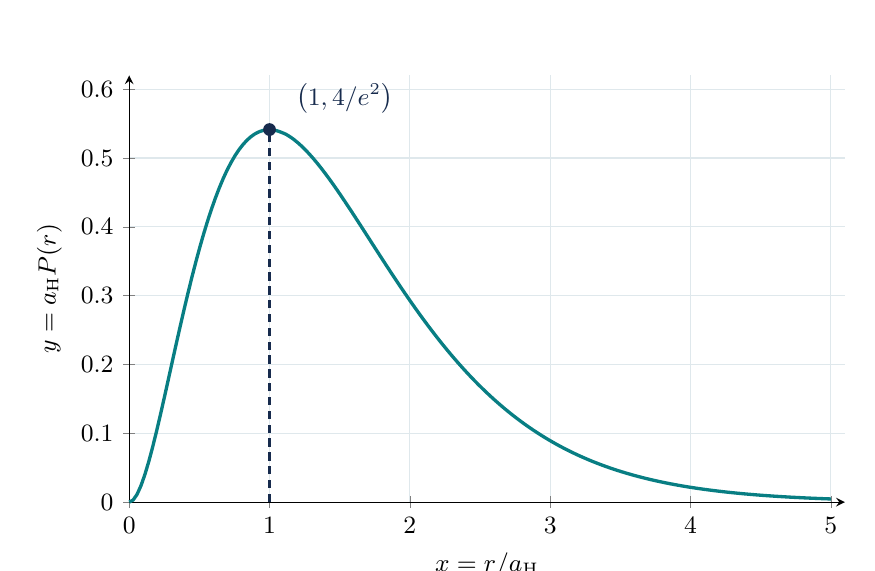
\begin{tikzpicture}
\begin{axis}[
 width=.88\textwidth,height=7cm,
 xmin=0,xmax=5.1,ymin=0,ymax=.62,
 xlabel={$x=r/\aH$},ylabel={$y=\aH P(r)$},
 axis lines=left,grid=both,major grid style={line!60},minor grid style={line!28},
 xtick={0,1,2,3,4,5},ytick={0,.1,.2,.3,.4,.5,.6},
 tick label style={font=\small},label style={font=\small},
 clip=false]
\addplot[teal,very thick,domain=0:5,samples=180] {4*x^2*exp(-2*x)};
\addplot[navy,densely dashed,thick] coordinates {(1,0) (1,0.541341132946)};
\addplot[only marks,mark=*,mark size=2.1pt,navy] coordinates {(1,0.541341132946)};
\node[anchor=south west,font=\small,color=navy] at (axis cs:1.12,.55) {$\left(1,4/e^2\right)$};
\end{axis}
\end{tikzpicture}
\caption{Normalized hydrogen \(1s\) radial probability density in dimensionless form \(\aH P(r)=4(r/\aH)^2e^{-2r/\aH}\). The unique global maximum is at \(r/\aH=1\).}
\label{fig:hydrogenradial}
\end{figure}

\subsubsection*{Step 6: Distinguish spatial and radial densities}
The \emph{spatial} density is \(\rho_{\rm spatial}(r)=|\psi_{100}|^2=(\pi\aH^3)^{-1}\ee^{-2r/\aH}\), with units \(L^{-3}\). Its derivative is negative for every \(r\ge0\), so its maximum is at \(r=0\). By contrast the \emph{radial} density is \(P(r)=4\pi r^2\rho_{\rm spatial}(r)\), with units \(L^{-1}\), which peaks at \(r=\aH\) because the shell-volume factor grows as \(r^2\). There is no contradiction. The cumulative probability inside radius \(b\) is
\begin{equation}\boxed{F(b)=\int_0^bP(r)\dd r=1-\ee^{-2b/\aH}\left(1+\frac{2b}{\aH}+\frac{2b^2}{\aH^2}\right).}\end{equation}
At \(b=\aH\), \(F(\aH)=1-5e^{-2}\simeq0.3233\). Thus the most probable radius does not enclose 50\% of the probability. The mean radius is \(\avg r=3\aH/2\) (B7), also distinct from the mode. The curve in Fig.~\ref{fig:hydrogenradial} and the negative second derivative establish the assignment claim.

\subsection{B9. Vanishing Cartesian position means in the hydrogen ground state}
\begin{questionbox}Show that \(\langle x\rangle=\langle y\rangle=\langle z\rangle=0\) for the ground state \((\psi_{100})\) of hydrogen atom.\end{questionbox}
\subsubsection*{Step 1: Normalized state and spherical coordinates}
The reduced-mass \(1s\) wavefunction is
\begin{equation}\psi_{100}(r)=\frac{\ee^{-r/\aH}}{\sqrt{\pi\aH^3}},\qquad |\psi_{100}|^2=\frac{\ee^{-2r/\aH}}{\pi\aH^3}.\end{equation}
As before, \((4/\aH^3)\int_0^\infty r^2\ee^{-2r/\aH}\dd r=1\). The operators act by multiplication. In spherical coordinates,
\begin{equation}x=r\sin\theta\cos\phi,\qquad y=r\sin\theta\sin\phi,\qquad z=r\cos\theta,\qquad\dd^3r=r^2\sin\theta\dd r\dd\theta\dd\phi.\end{equation}
For any Cartesian coordinate \(q\), \(\avg q=\int_{\R^3}q|\psi|^2\dd^3r\).

\subsubsection*{Step 2: Calculate \texorpdfstring{$\langle x\rangle$}{<x>}}
\begin{align}
\avg x&=\frac1{\pi\aH^3}\int_0^\infty r^3\ee^{-2r/\aH}\dd r\int_0^\pi\sin^2\theta\dd\theta\int_0^{2\pi}\cos\phi\dd\phi.
\end{align}
The finite radial moment is \(\int_0^\infty r^3\ee^{-2r/\aH}\dd r=3!/(2/\aH)^4=3\aH^4/8\). The polar integral equals \(\int_0^\pi\sin^2\theta\dd\theta=\pi/2\), while
\begin{equation}\int_0^{2\pi}\cos\phi\dd\phi=[\sin\phi]_0^{2\pi}=0.\end{equation}
Therefore \(\boxed{\avg x=0}\).

\subsubsection*{Step 3: Calculate \texorpdfstring{$\langle y\rangle$}{<y>}}
\begin{equation}\avg y=\frac1{\pi\aH^3}\int_0^\infty r^3\ee^{-2r/\aH}\dd r\int_0^\pi\sin^2\theta\dd\theta\int_0^{2\pi}\sin\phi\dd\phi.\end{equation}
Here \(\int_0^{2\pi}\sin\phi\dd\phi=[-\cos\phi]_0^{2\pi}=0\). Thus \(\boxed{\avg y=0}\).

\subsubsection*{Step 4: Calculate \texorpdfstring{$\langle z\rangle$}{<z>}}
\begin{equation}\avg z=\frac1{\pi\aH^3}\int_0^\infty r^3\ee^{-2r/\aH}\dd r\int_0^\pi\sin\theta\cos\theta\dd\theta\int_0^{2\pi}\dd\phi.\end{equation}
Now \(\int_0^\pi\sin\theta\cos\theta\dd\theta=\tfrac12[\sin^2\theta]_0^\pi=0\), while \(\int_0^{2\pi}\dd\phi=2\pi\). Hence \(\boxed{\avg z=0}\).
\key{\boxed{\avg x_{100}=\avg y_{100}=\avg z_{100}=0,\qquad\avg{\mathbf r}=\mathbf0.}}

\subsubsection*{Step 5: Independent parity argument}
The \(1s\) state is even under inversion: \(\psi_{100}(-\mathbf r)=\psi_{100}(\mathbf r)\). The position operators are odd: \(\mathcal P x_i\mathcal P^{-1}=-x_i\). Thus, changing variables \(\mathbf r\mapsto-\mathbf r\) in the expectation integral yields
\begin{equation}\avg{x_i}=\int x_i|\psi|^2\dd^3r=-\int x_i|\psi|^2\dd^3r=-\avg{x_i},\end{equation}
so \(\avg{x_i}=0\). In fact, every parity eigenstate with finite first position moments has this property.

\subsubsection*{Step 6: Rotational-symmetry argument and interpretation}
A rotationally invariant state has \(\psi(\mathcal R\mathbf r)=\psi(\mathbf r)\), so its mean vector must satisfy \(\mathcal R\avg{\mathbf r}=\avg{\mathbf r}\) for all \(\mathcal R\in SO(3)\). Only the zero vector has this property, proving \(\avg{\mathbf r}=0\). More explicitly, a \(\pi\)-rotation about \(z\) sends \((x,y,z)\mapsto(-x,-y,z)\), forcing \(\avg x=\avg y=0\); a \(\pi\)-rotation about \(x\) forces \(\avg z=0\).
This does \emph{not} imply that \(\avg r=0\): from B7, \(\avg r=3\aH/2>0\). The vector mean cancels directions, while radial distance is nonnegative. The integrals are absolutely convergent because \(r^3e^{-2r/\aH}\) is integrable near \(0\) and infinity. Thus the angular cancellation is legitimate.

\subsection{B10. Cartesian second moments and variances in the \texorpdfstring{$1s$}{1s} state}
\begin{questionbox}Show that \(\langle x^2\rangle=\langle y^2\rangle=\langle z^2\rangle=\tfrac13\langle r^2\rangle\) for the ground state \((\psi_{100})\) of hydrogen atom.\end{questionbox}
\subsubsection*{Step 1: Radial second moment}
For the normalized state \(|\psi|^2=(\pi\aH^3)^{-1}\ee^{-2r/\aH}\),
\begin{align}
\avg{r^2}&=\int_{\R^3}r^2|\psi|^2\dd^3r=\frac4{\aH^3}\int_0^\infty r^4\ee^{-2r/\aH}\dd r\\
&=\frac4{\aH^3}\frac{4!}{(2/\aH)^5}=\frac4{\aH^3}\frac{24\aH^5}{32}=3\aH^2.
\end{align}
Therefore \(\boxed{\avg{r^2}=3\aH^2}\). The normalized state check is \((4/\aH^3)\int r^2\ee^{-2r/\aH}\dd r=1\).

\subsubsection*{Step 2: Explicit \texorpdfstring{$x^2$}{x2} integral}
Since \(x^2=r^2\sin^2\theta\cos^2\phi\),
\begin{align}
\avg{x^2}&=\frac1{\pi\aH^3}\int_0^\infty r^4\ee^{-2r/\aH}\dd r\int_0^\pi\sin^3\theta\dd\theta\int_0^{2\pi}\cos^2\phi\dd\phi.
\end{align}
With \(u=\cos\theta\),
\begin{equation}\int_0^\pi\sin^3\theta\dd\theta=\int_{-1}^1(1-u^2)\dd u=\left[u-\frac{u^3}{3}\right]_{-1}^1=\frac43.\end{equation}
Using \(\cos^2\phi=(1+\cos2\phi)/2\), \(\int_0^{2\pi}\cos^2\phi\dd\phi=\pi\). Therefore
\begin{align}
\avg{x^2}&=\frac1{\pi\aH^3}\left(\frac{3\aH^5}{4}\right)\frac43\pi=\aH^2.
\end{align}
Thus \(\boxed{\avg{x^2}=\aH^2}\).

\subsubsection*{Step 3: Explicit \texorpdfstring{$y^2$}{y2} integral}
Since \(y^2=r^2\sin^2\theta\sin^2\phi\),
\begin{align}
\avg{y^2}&=\frac1{\pi\aH^3}\int_0^\infty r^4\ee^{-2r/\aH}\dd r\int_0^\pi\sin^3\theta\dd\theta\int_0^{2\pi}\sin^2\phi\dd\phi.
\end{align}
Here \(\int_0^{2\pi}\sin^2\phi\dd\phi=\pi\). Thus \(\avg{y^2}=(\pi\aH^3)^{-1}(3\aH^5/4)(4/3)\pi=\aH^2\), giving \(\boxed{\avg{y^2}=\aH^2}\).

\subsubsection*{Step 4: Explicit \texorpdfstring{$z^2$}{z2} integral}
Since \(z^2=r^2\cos^2\theta\),
\begin{align}
\avg{z^2}&=\frac1{\pi\aH^3}\int_0^\infty r^4\ee^{-2r/\aH}\dd r\int_0^\pi\cos^2\theta\sin\theta\dd\theta\int_0^{2\pi}\dd\phi.
\end{align}
With \(u=\cos\theta\),
\begin{equation}\int_0^\pi\cos^2\theta\sin\theta\dd\theta=\int_{-1}^1u^2\dd u=\frac23.\end{equation}
Thus \(\avg{z^2}=(\pi\aH^3)^{-1}(3\aH^5/4)(2/3)(2\pi)=\aH^2\), so \(\boxed{\avg{z^2}=\aH^2}\).

\subsubsection*{Step 5: Isotropy and tensor proof}
For any rotationally invariant probability law, the symmetric matrix \(M_{ij}=\avg{x_ix_j}\) obeys \(\mathcal R M\mathcal R^\mathsf T=M\) for every \(\mathcal R\in SO(3)\). Therefore \(M_{ij}=C\delta_{ij}\). Taking the trace,
\begin{equation}3C=\operatorname{Tr}M=\avg{x^2+y^2+z^2}=\avg{r^2},\qquad C=\frac13\avg{r^2}.\end{equation}
Thus, independently of the explicit radial function,
\key{\boxed{\avg{x^2}=\avg{y^2}=\avg{z^2}=\frac13\avg{r^2}=\aH^2.}}
Off-diagonal second moments also vanish: \(\avg{xy}=\avg{yz}=\avg{zx}=0\).

\subsubsection*{Step 6: Cartesian variances and uncertainty}
B9 established \(\avg x=\avg y=\avg z=0\). Therefore
\begin{equation}(\Delta x)^2=\avg{x^2}-(\avg x)^2=\aH^2,\end{equation}
with analogous formulas for \(y,z\). Hence
\key{\boxed{\Delta x=\Delta y=\Delta z=\aH\simeq5.29465\times10^{-11}\,\mathrm m\simeq0.529465\,\text{\AA}.}}
The covariance matrix is \(\Sigma_{ij}=\aH^2\delta_{ij}\). Note carefully that the radial standard deviation \(\Delta r=\sqrt3\aH/2\) differs from each Cartesian standard deviation. All second moments converge because \(r^4e^{-2r/\aH}\) is integrable at both ends, and all quantities have the correct dimensions.

\subsection{B11. Algebraic angular-momentum spectrum from commutators and ladder norms}
\begin{questionbox}Determine the eigenvalues of \(\hat L^2\) and \(\hat L_z\) using the algebraic theory of angular momentum.\end{questionbox}
\subsubsection*{Step 1: Commutation relations and Casimir operator}
The Hermitian angular momentum components satisfy
\begin{equation}\boxed{[L_i,L_j]=\iu\hbar\varepsilon_{ijk}L_k,\quad L_i^\dagger=L_i.}\end{equation}
Define \(L^2=L_x^2+L_y^2+L_z^2\). From the product commutator identity,
\begin{align}
[L^2,L_z]&=[L_x^2,L_z]+[L_y^2,L_z]\\
&=-\iu\hbar(L_xL_y+L_yL_x)+\iu\hbar(L_yL_x+L_xL_y)=0.
\end{align}
Cyclic permutations similarly give \([L^2,L_x]=[L^2,L_y]=0\). We may choose normalized common eigenvectors and, \emph{without assuming their eigenvalues}, write
\begin{equation}\boxed{L^2\ket{\lambda,\mu}=\hbar^2\lambda\ket{\lambda,\mu},\qquad L_z\ket{\lambda,\mu}=\hbar\mu\ket{\lambda,\mu}.}\end{equation}
Hermiticity implies \(\lambda,\mu\in\R\), and positivity gives \(\lambda\ge0\).

\subsubsection*{Step 2: Define ladders and prove their commutators}
Define \(L_\pm=L_x\pm\iu L_y\), with \(L_\pm^\dagger=L_\mp\). The angular commutation relations give
\begin{align}
[L_z,L_+]&=[L_z,L_x]+\iu[L_z,L_y]\\
&=\iu\hbar L_y+\iu(-\iu\hbar L_x)=\hbar L_+,\\
[L_z,L_-]&=[L_z,L_x]-\iu[L_z,L_y]=-\hbar L_-.
\end{align}
Thus \([L_z,L_\pm]=\pm\hbar L_\pm\). Since \([L^2,L_x]=[L^2,L_y]=0\), also \([L^2,L_\pm]=0\). Applying to \(\ket{\lambda,\mu}\),
\begin{align}
L_z(L_\pm\ket{\lambda,\mu})&=(L_\pm L_z\pm\hbar L_\pm)\ket{\lambda,\mu}\\
&=\hbar(\mu\pm1)L_\pm\ket{\lambda,\mu},\\
L^2(L_\pm\ket{\lambda,\mu})&=\hbar^2\lambda L_\pm\ket{\lambda,\mu}.
\end{align}
Hence the ladder changes \(\mu\mapsto\mu\pm1\) while preserving \(\lambda\), unless the result is the zero vector.

\subsubsection*{Step 3: Ordered products and norm positivity}
Direct multiplication without commuting the operators gives
\begin{align}
L_+L_-&=L_x^2+L_y^2-\iu[L_x,L_y]=L^2-L_z^2+\hbar L_z,\\
L_-L_+&=L_x^2+L_y^2+\iu[L_x,L_y]=L^2-L_z^2-\hbar L_z.
\end{align}
Since \(L_+^\dagger=L_-\),
\begin{align}
\norm{L_+\ket{\lambda,\mu}}^2&=\bra{\lambda,\mu}L_-L_+\ket{\lambda,\mu}=\hbar^2[\lambda-\mu(\mu+1)]\ge0,\\
\norm{L_-\ket{\lambda,\mu}}^2&=\bra{\lambda,\mu}L_+L_-\ket{\lambda,\mu}=\hbar^2[\lambda-\mu(\mu-1)]\ge0.
\end{align}
Also \(\avg{L_x^2+L_y^2}=\hbar^2(\lambda-\mu^2)\ge0\), so
\begin{equation}\boxed{\mu^2\le\lambda.}\end{equation}
This bound forbids infinitely many unit-raising or unit-lowering steps at fixed finite \(\lambda\). A highest and a lowest state must exist in the irreducible ladder.

\subsubsection*{Step 4: Highest and lowest weights}
Let \(\mu_{\max}\) and \(\mu_{\min}\) be the top and bottom values. Their ladder results vanish:
\begin{equation}L_+\ket{\lambda,\mu_{\max}}=0,\qquad L_-\ket{\lambda,\mu_{\min}}=0.\end{equation}
The squared-norm identities yield
\begin{equation}\boxed{\lambda=\mu_{\max}(\mu_{\max}+1)=\mu_{\min}(\mu_{\min}-1).}\end{equation}
Equate and factor:
\begin{align}
0&=\mu_{\max}(\mu_{\max}+1)-\mu_{\min}(\mu_{\min}-1)\\
&=(\mu_{\max}+\mu_{\min})(\mu_{\max}-\mu_{\min}+1).
\end{align}
The second factor is positive because \(\mu_{\max}\ge\mu_{\min}\); hence \(\mu_{\min}=-\mu_{\max}\).

\subsubsection*{Step 5: Quantization from the integer number of ladder steps}
Suppose there are \(N\ge0\) raising steps, so \(\mu_{\max}-\mu_{\min}=N\), with \(N\in\mathbb Z\). Since \(\mu_{\min}=-\mu_{\max}\),
\begin{equation}2\mu_{\max}=N.\end{equation}
Define \(j=N/2=\mu_{\max}\). Then
\begin{equation}\boxed{j=0,\frac12,1,\frac32,\ldots,\quad m=-j,-j+1,\ldots,j.}\end{equation}
The highest-weight condition gives \(\lambda=j(j+1)\). Consequently,
\key{\boxed{L^2\ket{j,m}=\hbar^2j(j+1)\ket{j,m},\qquad L_z\ket{j,m}=\hbar m\ket{j,m}.}}
The irreducible multiplet has \(2j+1\) magnetic states.

\subsubsection*{Step 6: Normalized ladder coefficients}
Write \(L_+\ket{j,m}=C_{jm}^+\ket{j,m+1}\). The norm calculation gives
\begin{align}
|C_{jm}^+|^2&=\hbar^2[j(j+1)-m(m+1)],\\
|C_{jm}^-|^2&=\hbar^2[j(j+1)-m(m-1)].
\end{align}
Choosing standard phases gives
\key{\boxed{L_\pm\ket{j,m}=\hbar\sqrt{j(j+1)-m(m\pm1)}\ket{j,m\pm1}.}}
At \(m=j\), \(L_+\ket{j,j}=0\); at \(m=-j\), \(L_-\ket{j,-j}=0\). The norms determine coefficient magnitudes, while state phases establish the chosen positive signs.

\subsubsection*{Step 7: Orbital versus half-integer spin}
The abstract algebra admits both integer and half-integer \(j\). For \emph{orbital} angular momentum \(\mathbf L=\mathbf r\times\mathbf p\) acting on scalar spatial functions, \(L_z=-\iu\hbar\partial_\phi\). Thus \(L_z\Phi=\hbar m\Phi\) has \(\Phi(\phi)\propto e^{\iu m\phi}\). Single-valuedness under \(\phi\mapsto\phi+2\pi\) requires \(m\in\mathbb Z\). Since the highest \(m=j\) must be an integer in an orbital multiplet,
\begin{equation}\boxed{l=0,1,2,\ldots,\qquad m=-l,\ldots,l,\quad L^2=\hbar^2l(l+1),\quad L_z=\hbar m.}\end{equation}
Half-integer spin is allowed because spinors transform under \(SU(2)\), the double cover of \(SO(3)\); a \(2\pi\) rotation changes a spin-\(1/2\) spinor's sign without changing the physical ray. In particular \(S^2=3\hbar^2/4\), \(S_z=\pm\hbar/2\) for electron spin. For \(l=1\), \(L^2=2\hbar^2\) and \(m=-1,0,1\), with \(L_+\ket{1,0}=\sqrt2\hbar\ket{1,1}\). This provides an explicit consistency check.

\subsection{B12. Derive spherical-coordinate angular momentum operators and spherical-harmonic eigenfunctions}
\begin{questionbox}Express the angular momentum operators in polar coordinates and prove that the spherical harmonics are the eigenfunctions of \(\hat L^2\) and \(\hat L_z\).\end{questionbox}
\subsubsection*{Step 1: From the vector definition to Cartesian operators}
Using \(\mathbf p=-\iu\hbar\nabla\),
\begin{equation}\boxed{\mathbf L=\mathbf r\times\mathbf p=-\iu\hbar(\mathbf r\times\nabla).}\end{equation}
The Cartesian components are
\begin{equation}\boxed{L_x=-\iu\hbar(y\p_z-z\p_y),\quad L_y=-\iu\hbar(z\p_x-x\p_z),\quad L_z=-\iu\hbar(x\p_y-y\p_x).}\end{equation}
The spherical coordinates are \(x=r\sin\theta\cos\phi\), \(y=r\sin\theta\sin\phi\), \(z=r\cos\theta\).

\subsubsection*{Step 2: Derive the multivariable chain rules}
For smooth \(f(r,\theta,\phi)\),
\begin{equation}\p_xf=(\p_xr)\p_rf+(\p_x\theta)\p_\theta f+(\p_x\phi)\p_\phi f,\end{equation}
with analogous expressions for \(y,z\). Since \(r=\sqrt{x^2+y^2+z^2}\), \(\cos\theta=z/r\), and \(\tan\phi=y/x\) locally,
\begin{equation}
\begin{array}{c|ccc}
&\p_x&\p_y&\p_z\\\hline
r&\sin\theta\cos\phi&\sin\theta\sin\phi&\cos\theta\\[1mm]
\theta&\cos\theta\cos\phi/r&\cos\theta\sin\phi/r&-\sin\theta/r\\[1mm]
\phi&-\sin\phi/(r\sin\theta)&\cos\phi/(r\sin\theta)&0
\end{array}
\end{equation}
For example, differentiating \(\cos\theta=z/r\) with respect to \(x\) gives \(-\sin\theta\,\p_x\theta=-zx/r^3\), hence \(\p_x\theta=\cos\theta\cos\phi/r\). Differentiating \(\operatorname{atan2}(y,x)\) gives \(\p_x\phi=-y/(x^2+y^2)\). Therefore,
\begin{align}
\p_x&=\sin\theta\cos\phi\,\p_r+\frac{\cos\theta\cos\phi}{r}\p_\theta-\frac{\sin\phi}{r\sin\theta}\p_\phi,\\
\p_y&=\sin\theta\sin\phi\,\p_r+\frac{\cos\theta\sin\phi}{r}\p_\theta+\frac{\cos\phi}{r\sin\theta}\p_\phi,\\
\p_z&=\cos\theta\,\p_r-\frac{\sin\theta}{r}\p_\theta.
\end{align}

\subsubsection*{Step 3: Calculate \texorpdfstring{$L_x,L_y,L_z$}{Lx Ly Lz}}
For \(L_x=-\iu\hbar(y\p_z-z\p_y)\), substitute \(y=r\sin\theta\sin\phi\), \(z=r\cos\theta\). Then
\begin{align}
y\p_z&=r\sin\theta\cos\theta\sin\phi\,\p_r-\sin^2\theta\sin\phi\,\p_\theta,\\
z\p_y&=r\sin\theta\cos\theta\sin\phi\,\p_r+\cos^2\theta\sin\phi\,\p_\theta+\cot\theta\cos\phi\,\p_\phi.
\end{align}
The radial derivatives cancel, giving
\begin{equation}\boxed{L_x=\iu\hbar(\sin\phi\,\p_\theta+\cot\theta\cos\phi\,\p_\phi).}\end{equation}
Likewise,
\begin{align}
z\p_x&=r\sin\theta\cos\theta\cos\phi\,\p_r+\cos^2\theta\cos\phi\,\p_\theta-\cot\theta\sin\phi\,\p_\phi,\\
x\p_z&=r\sin\theta\cos\theta\cos\phi\,\p_r-\sin^2\theta\cos\phi\,\p_\theta,
\end{align}
so
\begin{equation}\boxed{L_y=\iu\hbar(-\cos\phi\,\p_\theta+\cot\theta\sin\phi\,\p_\phi).}\end{equation}
Finally, direct substitution gives \(x\p_y-y\p_x=(\cos^2\phi+\sin^2\phi)\p_\phi=\p_\phi\), hence
\begin{equation}\boxed{L_z=-\iu\hbar\p_\phi.}\end{equation}
All three lack \(\p_r\), because angular momentum generates changes of direction at fixed radius.

\subsubsection*{Step 4: Ladder operators}
From \(L_\pm=L_x\pm\iu L_y\) and \(e^{\pm\iu\phi}=\cos\phi\pm\iu\sin\phi\),
\begin{equation}\boxed{L_\pm=\hbar\ee^{\pm\iu\phi}\left(\pm\p_\theta+\iu\cot\theta\,\p_\phi\right).}\end{equation}
For example,
\begin{align}
L_+&=\iu\hbar(\sin\phi\p_\theta+\cot\theta\cos\phi\p_\phi)-\hbar(-\cos\phi\p_\theta+\cot\theta\sin\phi\p_\phi)\\
&=\hbar(\cos\phi+\iu\sin\phi)\p_\theta+\iu\hbar\cot\theta(\cos\phi+\iu\sin\phi)\p_\phi.
\end{align}
The lowering formula follows by the opposite sign.

\subsubsection*{Step 5: Compute \texorpdfstring{$L^2$}{L squared} with coefficient derivatives}
Write \(L_x=\iu\hbar A\), \(L_y=\iu\hbar B\), where \(A=\sin\phi\p_\theta+\cot\theta\cos\phi\p_\phi\) and \(B=-\cos\phi\p_\theta+\cot\theta\sin\phi\p_\phi\). Acting on an arbitrary smooth angular function \(f\), the product rule gives
\begin{equation}A^2+B^2=\p_\theta^2+\cot\theta\p_\theta+\cot^2\theta\p_\phi^2.\end{equation}
The mixed derivatives cancel: their coefficient is \(2\cot\theta(\sin\phi\cos\phi-\cos\phi\sin\phi)=0\). First-order \(\p_\phi\) terms also cancel, including derivatives of \(\cot\theta\); the first-order \(\p_\theta\) coefficient is \(\cot\theta(\cos^2\phi+\sin^2\phi)=\cot\theta\). Since \(L_z^2=-\hbar^2\p_\phi^2\),
\begin{align}
L^2&=-\hbar^2[A^2+B^2+\p_\phi^2]\\
&=-\hbar^2\left[\p_\theta^2+\cot\theta\p_\theta+\csc^2\theta\p_\phi^2\right]\\
&=\boxed{-\hbar^2\left[\frac1{\sin\theta}\p_\theta(\sin\theta\p_\theta)+\frac1{\sin^2\theta}\p_\phi^2\right]}.
\end{align}
The expression in brackets is the Laplace--Beltrami operator \(\Delta_{S^2}\) on the unit sphere, so \(L^2=-\hbar^2\Delta_{S^2}\).

\subsubsection*{Step 6: Derive angular eigenfunctions}
Separate \(Y(\theta,\phi)=\Theta(\theta)\Phi(\phi)\). The \(L_z\) eigenvalue equation \(-\iu\hbar\Phi'=\hbar m\Phi\) gives \(\Phi\propto e^{\iu m\phi}\); periodicity forces \(m\in\mathbb Z\). The \(L^2\) equation \(L^2Y=\hbar^2\lambda Y\) reduces to
\begin{equation}\frac1{\sin\theta}\frac{\dd}{\dd\theta}(\sin\theta\Theta')+\left(\lambda-\frac{m^2}{\sin^2\theta}\right)\Theta=0.\end{equation}
With \(u=\cos\theta\), this becomes \((1-u^2)\Theta''-2u\Theta'+[\lambda-m^2/(1-u^2)]\Theta=0\). Smoothness at both poles selects \(\lambda=l(l+1)\) and \(\Theta\propto P_l^m(\cos\theta)\), \(l\in\mathbb N_0\), \(|m|\le l\). The normalized angular functions (Condon--Shortley convention) are
\begin{equation}\boxed{Y_l^m(\theta,\phi)=N_{lm}P_l^m(\cos\theta)e^{\iu m\phi},\quad N_{lm}=\sqrt{\frac{2l+1}{4\pi}\frac{(l-m)!}{(l+m)!}}.}\end{equation}
For \(m\ge0\), \(P_l^m(u)=(-1)^m(1-u^2)^{m/2}\dd^mP_l/\dd u^m\), where \(P_l(u)=(2^ll!)^{-1}(\dd/\dd u)^l(u^2-1)^l\). The angular measure is \(\dd\Omega=\sin\theta\dd\theta\dd\phi\), and \(\int Y_l^{m*}Y_{l'}^{m'}\dd\Omega=\delta_{ll'}\delta_{mm'}\).

\subsubsection*{Step 7: Prove the two eigenvalue equations}
First,
\begin{align}
L_zY_l^m&=-\iu\hbar\p_\phi[N_{lm}P_l^m(\cos\theta)e^{\iu m\phi}]\\
&=\hbar mY_l^m.
\end{align}
Second, the associated Legendre equation implies
\begin{equation}\frac1{\sin\theta}\frac{\dd}{\dd\theta}\left(\sin\theta\frac{\dd P_l^m}{\dd\theta}\right)-\frac{m^2}{\sin^2\theta}P_l^m=-l(l+1)P_l^m.\end{equation}
Since \(\p_\phi^2e^{\iu m\phi}=-m^2e^{\iu m\phi}\), applying \(L^2\) gives
\begin{align}
L^2Y_l^m&=-\hbar^2N_{lm}e^{\iu m\phi}\left[\frac1{\sin\theta}\frac{\dd}{\dd\theta}(\sin\theta\frac{\dd P_l^m}{\dd\theta})-\frac{m^2}{\sin^2\theta}P_l^m\right]\\
&=\hbar^2l(l+1)Y_l^m.
\end{align}
\key{\boxed{L^2Y_l^m=\hbar^2l(l+1)Y_l^m,\qquad L_zY_l^m=\hbar mY_l^m.}}

\subsubsection*{Step 8: Prove the ladder action}
Apply \(L_+=\hbar e^{\iu\phi}(\p_\theta+\iu\cot\theta\p_\phi)\):
\begin{equation}L_+Y_l^m=\hbar N_{lm}e^{\iu(m+1)\phi}\left[\frac{\dd P_l^m(\cos\theta)}{\dd\theta}-m\cot\theta P_l^m(\cos\theta)\right].\end{equation}
The associated Legendre identity \((\dd/\dd\theta-m\cot\theta)P_l^m(\cos\theta)=P_l^{m+1}(\cos\theta)\), combined with \(N_{lm}/N_{l,m+1}=\sqrt{(l-m)(l+m+1)}\), yields
\begin{equation}\boxed{L_+Y_l^m=\hbar\sqrt{(l-m)(l+m+1)}Y_l^{m+1}.}\end{equation}
The corresponding lowering identity \((-\dd/\dd\theta-m\cot\theta)P_l^m=(l+m)(l-m+1)P_l^{m-1}\) gives
\begin{equation}\boxed{L_-Y_l^m=\hbar\sqrt{(l+m)(l-m+1)}Y_l^{m-1}.}\end{equation}
Thus \(L_\pm Y_l^m=\hbar\sqrt{l(l+1)-m(m\pm1)}Y_l^{m\pm1}\); the top \(m=l\) and bottom \(m=-l\) states are annihilated.

\subsubsection*{Step 9: Explicit \texorpdfstring{$l=1$}{l=1} verification}
The normalized functions are
\begin{equation}Y_1^0=\sqrt{\frac3{4\pi}}\cos\theta,\quad Y_1^1=-\sqrt{\frac3{8\pi}}\sin\theta e^{\iu\phi},\quad Y_1^{-1}=+\sqrt{\frac3{8\pi}}\sin\theta e^{-\iu\phi}.\end{equation}
For \(f=\cos\theta\), \(f''+\cot\theta f'=-2\cos\theta\), giving \(L^2Y_1^0=2\hbar^2Y_1^0\). Also \(L_zY_1^1=-\iu\hbar(\iu)Y_1^1=\hbar Y_1^1\). Direct differentiation gives
\begin{align}
L_+Y_1^0&=\hbar e^{\iu\phi}\p_\theta\left(\sqrt{\frac3{4\pi}}\cos\theta\right)=-\hbar\sqrt{\frac3{4\pi}}\sin\theta e^{\iu\phi}=\sqrt2\hbar Y_1^1,\\
L_-Y_1^0&=\sqrt2\hbar Y_1^{-1},\qquad L_+Y_1^1=0,\quad L_-Y_1^{-1}=0.
\end{align}

\subsubsection*{Step 10: Explicit \texorpdfstring{$l=2$}{l=2} verification}
\begin{align}
Y_2^0&=\sqrt{\frac5{16\pi}}(3\cos^2\theta-1),\\
Y_2^1&=-\sqrt{\frac{15}{8\pi}}\sin\theta\cos\theta\,e^{\iu\phi},\\
Y_2^2&=\sqrt{\frac{15}{32\pi}}\sin^2\theta\,e^{2\iu\phi}.
\end{align}
For \(f=3\cos^2\theta-1\), \(f'=-6\sin\theta\cos\theta\), \(f''=-6(\cos^2\theta-\sin^2\theta)\), and \(f''+\cot\theta f'=-6f\). Hence \(L^2Y_2^0=6\hbar^2Y_2^0\). Likewise \(L_zY_2^2=2\hbar Y_2^2\) and \(L^2Y_2^2=6\hbar^2Y_2^2\). Applying the raising operator,
\begin{align}
L_+Y_2^0&=-6\hbar\sqrt{\frac5{16\pi}}\sin\theta\cos\theta e^{\iu\phi}=\sqrt6\hbar Y_2^1,\\
L_+Y_2^1&=\hbar\sqrt{\frac{15}{8\pi}}\sin^2\theta e^{2\iu\phi}=2\hbar Y_2^2.
\end{align}
Similarly \(L_-Y_2^2=2\hbar Y_2^1\), \(L_+Y_2^2=0\), \(L_-Y_2^{-2}=0\). These explicitly verify the differential formulas and match the algebraic spectrum B11.

\subsubsection*{Domain and self-adjointness check}
The angular Hilbert space is \(L^2(S^2,\dd\Omega)\). On smooth globally regular scalar functions,
\begin{equation}\langle f|L^2f\rangle=\hbar^2\int_{S^2}\left(|\p_\theta f|^2+\frac{|\p_\phi f|^2}{\sin^2\theta}\right)\dd\Omega\ge0.\end{equation}
Integration-by-parts surface terms vanish because the sphere has no boundary and smoothness handles coordinate poles. The apparent \(\cot\theta\), \(\csc\theta\) singularities arise from coordinate charts, not physical singularities of \(L_i\). This completes the operator and eigenfunction derivation.

\subsection{B13. Conservation of angular momentum in a spherically symmetric potential}
\begin{questionbox}Show that \(\displaystyle\frac{\dd\langle\mathbf L\rangle}{\dd t}=0\) for any spherically symmetric potential.\end{questionbox}
\subsubsection*{Step 1: State the Hamiltonian and canonical algebra}
For a spinless particle with a scalar central potential,
\begin{equation}\boxed{H=T+V(r)=\frac{p_x^2+p_y^2+p_z^2}{2\mu}+V(r),\qquad r=\sqrt{x^2+y^2+z^2}.}\end{equation}
The components of orbital angular momentum are
\begin{equation}L_x=yp_z-zp_y,\qquad L_y=zp_x-xp_z,\qquad L_z=xp_y-yp_x.\end{equation}
The canonical commutators are \([x_i,p_j]=\iu\hbar\delta_{ij}\), \([x_i,x_j]=[p_i,p_j]=0\). For a differentiable multiplication operator \(f(\mathbf r)\),
\begin{equation}\boxed{[p_i,f]=-\iu\hbar\p_i f,\qquad[f,p_i]=\iu\hbar\p_i f.}\end{equation}
To prove conservation, it suffices to show \([H,L_i]=[T,L_i]+[V,L_i]=0\) for each \(i\).

\subsubsection*{Step 2: Explicit kinetic commutator with \texorpdfstring{$L_x$}{Lx}}
Using \(L_x=yp_z-zp_y\),
\begin{equation}[p_x,L_x]=0,\qquad[p_y,L_x]=-\iu\hbar p_z,\qquad[p_z,L_x]=\iu\hbar p_y.\end{equation}
Apply \([A^2,B]=A[A,B]+[A,B]A\):
\begin{align}
[p_x^2,L_x]&=0,\\
[p_y^2,L_x]&=-\iu\hbar(p_yp_z+p_zp_y),\\
[p_z^2,L_x]&=+\iu\hbar(p_zp_y+p_yp_z).
\end{align}
Adding, \([p_x^2+p_y^2+p_z^2,L_x]=0\); thus
\begin{equation}\boxed{[T,L_x]=0.}\end{equation}

\subsubsection*{Step 3: Explicit kinetic commutator with \texorpdfstring{$L_y$}{Ly}}
For \(L_y=zp_x-xp_z\),
\begin{equation}[p_x,L_y]=\iu\hbar p_z,\qquad[p_y,L_y]=0,\qquad[p_z,L_y]=-\iu\hbar p_x.\end{equation}
Consequently,
\begin{align}
[p_x^2,L_y]&=+\iu\hbar(p_xp_z+p_zp_x),\\
[p_y^2,L_y]&=0,\\
[p_z^2,L_y]&=-\iu\hbar(p_zp_x+p_xp_z).
\end{align}
The terms cancel, giving \(\boxed{[T,L_y]=0}\).

\subsubsection*{Step 4: Explicit kinetic commutator with \texorpdfstring{$L_z$}{Lz}}
For \(L_z=xp_y-yp_x\),
\begin{equation}[p_x,L_z]=-\iu\hbar p_y,\qquad[p_y,L_z]=\iu\hbar p_x,\qquad[p_z,L_z]=0.\end{equation}
Therefore,
\begin{align}
[p_x^2,L_z]&=-\iu\hbar(p_xp_y+p_yp_x),\\
[p_y^2,L_z]&=+\iu\hbar(p_yp_x+p_xp_y),\\
[p_z^2,L_z]&=0.
\end{align}
Thus \(\boxed{[T,L_z]=0}\). Collecting,
\begin{equation}\boxed{[T,L_x]=[T,L_y]=[T,L_z]=0.}\end{equation}
The kinetic energy depends only on the rotational scalar \(\mathbf p^2\) and is invariant under all three rotations.

\subsubsection*{Step 5: Potential commutators by chain rule}
For a radial function,
\begin{equation}\boxed{\p_xV=V'(r)\frac xr,\quad \p_yV=V'(r)\frac yr,\quad \p_zV=V'(r)\frac zr.}\end{equation}
Since coordinates commute with \(V(r)\),
\begin{align}
[V,L_x]&=[V,yp_z-zp_y]=y[V,p_z]-z[V,p_y]\\
&=\iu\hbar(y\p_zV-z\p_yV)\\
&=\iu\hbar\frac{V'(r)}r(yz-zy)=0,\\[3pt]
[V,L_y]&=[V,zp_x-xp_z]=\iu\hbar(z\p_xV-x\p_zV)\\
&=\iu\hbar\frac{V'(r)}r(zx-xz)=0,\\[3pt]
[V,L_z]&=[V,xp_y-yp_x]=\iu\hbar(x\p_yV-y\p_xV)\\
&=\iu\hbar\frac{V'(r)}r(xy-yx)=0.
\end{align}
Therefore,
\begin{equation}\boxed{[V(r),L_x]=[V(r),L_y]=[V(r),L_z]=0.}\end{equation}
This uses only the radial dependence of \(V\), not any particular form such as Coulomb or oscillator. Singular potentials require suitable domains; a rotationally invariant self-adjoint Hamiltonian suffices for the global symmetry argument below.

\subsubsection*{Step 6: Hamiltonian commutators and Heisenberg conservation}
Combining the independent kinetic and potential calculations,
\key{\boxed{[H,L_x]=[H,L_y]=[H,L_z]=0.}}
For an operator without explicit Schr\"odinger-picture time dependence, the Heisenberg equation is
\begin{equation}\boxed{\frac{\dd A_H}{\dd t}=\frac{\iu}{\hbar}[H_H,A_H].}\end{equation}
Thus for each angular momentum component,
\begin{equation}\frac{\dd L_{i,H}}{\dd t}=\frac{\iu}{\hbar}[H_H,L_{i,H}]=0,\end{equation}
which integrates to \(L_{i,H}(t)=L_{i,H}(0)\). This is the stronger \emph{operator conservation law}.

\subsubsection*{Step 7: Expectation-value conservation}
Ehrenfest's equation for a Schr\"odinger-picture observable with no explicit time dependence is
\begin{equation}\frac{\dd}{\dd t}\avg A=\frac{\iu}{\hbar}\avg{[H,A]}.\end{equation}
Applying it to \(L_x,L_y,L_z\) and using their vanishing Hamiltonian commutators,
\begin{equation}\frac{\dd\avg{L_x}}{\dd t}=\frac{\dd\avg{L_y}}{\dd t}=\frac{\dd\avg{L_z}}{\dd t}=0.\end{equation}
Consequently,
\key{\boxed{\frac{\dd}{\dd t}\avg{\mathbf L}=\mathbf0,\qquad\avg{\mathbf L}(t)=\avg{\mathbf L}(0).}}
This holds for every normalizable state for which the relevant expectations exist, not only an energy eigenstate.

\subsubsection*{Step 8: Conservation of \texorpdfstring{$L^2$}{L squared}}
Since \(L^2=L_x^2+L_y^2+L_z^2\) and \([H,L_i]=0\),
\begin{align}
[H,L^2]&=\sum_i[H,L_i^2]\\
&=\sum_i([H,L_i]L_i+L_i[H,L_i])=0.
\end{align}
Hence \(\boxed{[H,L^2]=0}\), \(\dd L_H^2/\dd t=0\), and \(\dd\avg{L^2}/\dd t=0\). Because \([L^2,L_z]=0\), the operators \(H,L^2,L_z\) admit a common eigenbasis on the central-potential bound-state space, with \(\psi_{n_r l m}(r,\theta,\phi)=R_{n_r l}(r)Y_l^m(\theta,\phi)\).

\subsubsection*{Step 9: Classical zero torque and quantum correspondence}
The classical central force is \(\mathbf F=-\nabla V=-V'(r)\hat{\mathbf r}\). Differentiate \(\mathbf L=\mathbf r\times\mathbf p\):
\begin{align}
\frac{\dd\mathbf L}{\dd t}&=\dot{\mathbf r}\times\mathbf p+\mathbf r\times\dot{\mathbf p}\\
&=\dot{\mathbf r}\times\mu\dot{\mathbf r}+\mathbf r\times\mathbf F\\
&=\mathbf r\times[-V'(r)\hat{\mathbf r}]=\mathbf0.
\end{align}
Thus the central force produces zero torque. The quantum Heisenberg analogue is \(\dd\mathbf L_H/\dd t=-\mathbf r_H\times\nabla V(r_H)=\mathbf0\).

\subsubsection*{Step 10: Rotational symmetry and Noether theorem}
A rotation \(\mathcal R\) preserves \(r\) and \(\mathbf p^2\), hence leaves \(H\) invariant. Quantum rotation operators are generated by angular momentum:
\begin{equation}U(\vartheta)=\exp[-\iu\vartheta\,\mathbf n\cdot\mathbf L/\hbar].\end{equation}
Rotational invariance means \(U(\vartheta)^\dagger H U(\vartheta)=H\). Differentiate at \(\vartheta=0\):
\begin{equation}[H,\mathbf n\cdot\mathbf L]=0.\end{equation}
Since \(\mathbf n\) is arbitrary, \([H,L_i]=0\) for all components. The classical Lagrangian \(\mathscr L=\mu\dot{\mathbf r}^{\,2}/2-V(r)\) is also rotation invariant. For the infinitesimal transformation \(\delta\mathbf r=\delta\vartheta\,\mathbf n\times\mathbf r\), Noether's charge is
\begin{equation}Q_{\mathbf n}=\frac{\p\mathscr L}{\p\dot{\mathbf r}}\cdot\frac{\delta\mathbf r}{\delta\vartheta}=\mathbf p\cdot(\mathbf n\times\mathbf r)=\mathbf n\cdot(\mathbf r\times\mathbf p)=\mathbf n\cdot\mathbf L.\end{equation}
It is conserved for every \(\mathbf n\). Therefore continuous spatial rotational invariance entails angular momentum conservation.

\subsubsection*{Step 11: Physical caveats and interpretation}
Operator conservation \(\dd L_{i,H}/\dd t=0\) implies conservation of the expectation for every appropriate state, whereas a constant expectation in a single special state does not itself prove an operator commutator vanishes. Although the three components are each conserved, they do \emph{not} commute with each other: \([L_x,L_y]=\iu\hbar L_z\), so their simultaneous values need not all be sharp. For rotationally invariant \emph{spin-dependent} interactions such as \(f(r)\mathbf L\cdot\mathbf S\), total \(\mathbf J=\mathbf L+\mathbf S\) may be conserved while orbital \(\mathbf L\) separately is not; our proof assumes the specified spinless scalar Hamiltonian.

\textbf{Exam-ready conclusion.} The two independent commutator calculations give \([T,L_i]=[V(r),L_i]=0\), hence \([H,L_i]=0\). The Heisenberg--Ehrenfest equation then yields
\begin{equation}\boxed{\frac{\dd}{\dd t}\avg{\mathbf L}=\frac{\iu}{\hbar}\avg{[H,\mathbf L]}=\mathbf0.}\end{equation}
Thus orbital angular momentum is conserved in any spherically symmetric scalar potential. \textbf{Hence proved.}

\clearpage
\section{Consolidated results and examination checklist}
\begin{longtable}{p{.10\textwidth}p{.41\textwidth}p{.41\textwidth}}
\toprule
\textbf{Problem}&\textbf{Principal result}&\textbf{Key method}\tabularnewline\midrule\endfirsthead
\toprule\textbf{Problem}&\textbf{Principal result}&\textbf{Key method}\tabularnewline\midrule\endhead
A1 & \(V(\mathcal R\mathbf r)=V(\mathbf r)\) & Rotation preserves \(r\).\\
A2 & \(m\in\mathbb Z\) & Periodicity of \(e^{\iu m\phi}\).\\
A3 & Angular and hydrogen Kronecker orthonormality & Integrate with \(\dd\Omega\), \(r^2\dd r\dd\Omega\).\\
A4 & \(Y_l^{-m}=(-1)^m(Y_l^m)^*\) in standard convention & State the chosen phase convention.\\
A5 & \(E_n=-\mu Z^2e^4/[2(4\pi\eps)^2\hbar^2n^2]\) & Coulomb quantization.\\
A6 & \(\psi_{100}=(\pi a^3)^{-1/2}e^{-r/a}\) & Radial normalization.\\
A7 & \(\lambda^{-1}=R(1/n_f^2-1/n_i^2)\) & Photon energy conservation.\\
A8 & Seven operator commutators & Canonical algebra and products.\\
A9 & \(L^2=L_\pm L_\mp+L_z^2\mp\hbar L_z\) & Ordered ladder products.\\
A10 & \(\hbar\sqrt{l(l+1)-m(m\pm1)}\) & Positive squared norms.\\
B1 & Separated radial, \(\theta\), \(\phi\) equations & Spherical Laplacian, product ansatz.\\
B2 & \(P_l^m(\cos\theta)e^{\iu m\phi}\) & Associated Legendre equation.\\
B3 & \(E_{n0}=n^2\pi^2\hbar^2/(2\mu a^2)\) & Spherical Bessel/Dirichlet boundary.\\
B4 & \(P(r\le a/2)=1/2\) & 3D Born-rule radial integral.\\
B5 & \(E_n=-\mu g^2/(2\hbar^2n^2)\) & Frobenius series, polynomial termination.\\
B6 & \(\avg V_{1s}=-g/\aH=2E_1\) & 3D integral and virial theorem.\\
B7 & \(\Delta r=\sqrt3\aH/2\) & First and second radial moments.\\
B8 & \(r_{\rm mp}=\aH\) & Product derivative and second derivative.\\
B9 & \(\avg x=\avg y=\avg z=0\) & Angular integrals, parity, rotations.\\
B10 & \(\avg{x_i x_j}=\aH^2\delta_{ij}\) & Angular moments and isotropic tensor.\\
B11 & \(L^2=\hbar^2l(l+1),\ L_z=\hbar m\) & Ladder termination and norm positivity.\\
B12 & \(L^2=-\hbar^2\Delta_{S^2}\) & Multivariable chain rule and harmonics.\\
B13 & \([H,L_i]=0\Rightarrow\dd\avg{L_i}/\dd t=0\) & Explicit commutators and Noether.\\
\bottomrule
\end{longtable}
\textbf{Useful standard identities:}
\begin{align*}
&\int_0^\infty r^k\ee^{-\beta r}\dd r=\frac{\Gamma(k+1)}{\beta^{k+1}},\quad\beta>0,\ k>-1,\\
&\int_0^\pi\sin\theta\dd\theta=2,\quad\int_0^{2\pi}\dd\phi=2\pi,\quad\int_0^\pi\sin^3\theta\dd\theta=\frac43,\\
&\int_0^{2\pi}\sin^2\phi\dd\phi=\int_0^{2\pi}\cos^2\phi\dd\phi=\pi,\\
&[A,BC]=[A,B]C+B[A,C],\quad[AB,C]=A[B,C]+[A,C]B,\\
&[x_i,p_j]=\iu\hbar\delta_{ij},\quad[L_i,L_j]=\iu\hbar\varepsilon_{ijk}L_k.
\end{align*}

\section*{Closing note}
The manuscript is organized to be compiled directly with \texttt{pdflatex} in a standard TeX Live installation. It contains the complete Assignment IV question set (Part A: 10; Part B: 13), worked calculations, checks, and an analytic plot. It is a course-study artifact; arXiv-inspired typography does not imply arXiv submission, endorsement or independent research novelty.
\end{document}